\chapter{RESULTADOS DE 2 Y 3 QUBITS}
\janote{\textbf{Idea principal del capítulo:} los resultados gritan que los 
canales PCE sí se pueden caracterizar, pero nos hace falta LA idea (la de 
Francois, jajaja) para poder formalizar la caracterización general. Para mientras,
tenemos un listado de características que tienen sustento en los resultados
numéricos.}
\section{Introducción}

\section{Resultados}
%\noindent
%\esqueleto{Con el método numérico descrito en la sección 
%\ref{sec:ch2_solucionNumerica} es posible analizar el caso de 2 qubits
%completo. Por otro lado, el caso de 3 qubits es imposible de resolver 
%completo a fuerza bruta.}

En esta sección vamos a presentar los canales cuánticos PCE de 2 y 3 qubits 
encontrados con el método numérico descrito en la sección 
\ref{sec:ch2_solucionNumerica}. 
Por un lado, de las $32,768$ $(2^{15})$ operaciones PCE de 2 qubits, 
$67$ son canales cuánticos. La proporción $67:32,768$, de canales cuánticos PCE
a operaciones PCE, es evidencia de lo restrictivo
que es la condición de completa positividad para que una operación PCE 
sea una operación físicamente realizable. 
Por otro lado, las operaciones PCE de 3 qubits las estudiamos parcialmente.
Recordemos que el método numérico evalúa, una por una, la completa positividad 
de cada operación PCE y que el número de operaciónes PCE de $n$ qubits es igual
a $2^{4^n-1}$. Discutiremos en esta sección cómo es que nuestro 
método numérico necesitaría demasiado tiempo de cómputo y demasiada 
memoria para analizar la completa positividad de las $2^{63}$ 
operaciones PCE de 3 qubits.

%\noindent
%\esqueleto{Los resultados de 2 qubits son... (una tabla con 
%las listas de 1's y 0's de $\tau_{ij}$ por número $k$ de componentes 
%de Pauli invariantes). «\textit{La idea con esta tabla es motivar las 
%figuritas de la siguiente sección porque las listas de 1's y 0's no dicen 
%ni madres.}»}

En la \Tref{tab:2qubitsPCEChannel1sAnd0s} mostramos los canales 
cuánticos PCE de 2 qubits. En la tabla se muestran: 
(1) los valores de los elementos $\tau_{ij}$ (1 o 0) que caracterizan 
a una operación PCE, según la definición en \eqref{eq:PCE_definition},
y (2) el número de componentes de Pauli que el canal PCE
deja invariantes. Es difícil identificar características de los canales 
PCE de 2 qubits a partir de las listas de 1's y 0's en la tabla. 
Además, los sistemas de más de 1 qubit no cuentan con una herramienta 
geométrica, como la esfera de Bloch para 1 qubit, 
con la cual visualizar los estados del sistema y, en consecuencia, entender y 
desarrollar intuición sobre la acción de las operaciones PCE. 
En concolusión, es deseable elaborar una herramienta
que permita visualizar los resultados de la \Tref{tab:2qubitsPCEChannel1sAnd0s}
de una forma más sencilla. Hablaremos de una herramienta geométrica
en la próxima sección.

\begin{center}
\tiny 
\begin{longtable}{|P{0.3cm}|P{0.3cm}|P{0.3cm}|P{0.3cm}|P{0.3cm}|P{0.3cm}|P{0.3cm}|P{0.3cm}|P{0.3cm}|P{0.3cm}|P{0.3cm}|P{0.3cm}|P{0.3cm}|P{0.3cm}|P{0.3cm}|P{0.3cm}|P{0.3cm}|P{1.4cm}|}
\hline
\textbf{No.} 										 & \tauij{0}{0}		& \tauij{0}{1}   & \tauij{0}{2} 	 & \tauij{0}{3} 	& \tauij{1}{0}	 & \tauij{1}{1}		 & \tauij{1}{2} 	& \tauij{1}{3}	 & \tauij{2}{0}		& \tauij{2}{1} 		& \tauij{2}{2} 	 & \tauij{2}{3} 	& \tauij{3}{0} 	 & \tauij{3}{1}   & \tauij{3}{2}   & \tauij{3}{3} & \bf{Cantidad de \boldmath{$r_{ij}$} invariantes} \\ \hline
\textbf{1}                         & 1                     & 0                     & 0                     & 0                     & 0                     & 0                     & 0                     & 0                     & 0                     & 0                     & 0                     & 0                     & 0                     & 0                     & 0                     & 0                     & 1                     \\ \hline
\textbf{2}                         & 1                     & 1                     & 0                     & 0                     & 0                     & 0                     & 0                     & 0                     & 0                     & 0                     & 0                     & 0                     & 0                     & 0                     & 0                     & 0                     & 2                     \\ \hline
\textbf{3}                         & 1                     & 0                     & 1                     & 0                     & 0                     & 0                     & 0                     & 0                     & 0                     & 0                     & 0                     & 0                     & 0                     & 0                     & 0                     & 0                     & 2                     \\ \hline
\textbf{4}                         & 1                     & 0                     & 0                     & 1                     & 0                     & 0                     & 0                     & 0                     & 0                     & 0                     & 0                     & 0                     & 0                     & 0                     & 0                     & 0                     & 2                     \\ \hline
\textbf{5}                         & 1                     & 0                     & 0                     & 0                     & 1                     & 0                     & 0                     & 0                     & 0                     & 0                     & 0                     & 0                     & 0                     & 0                     & 0                     & 0                     & 2                     \\ \hline
\textbf{6}                         & 1                     & 0                     & 0                     & 0                     & 0                     & 1                     & 0                     & 0                     & 0                     & 0                     & 0                     & 0                     & 0                     & 0                     & 0                     & 0                     & 2                     \\ \hline
\textbf{7}                         & 1                     & 0                     & 0                     & 0                     & 0                     & 0                     & 1                     & 0                     & 0                     & 0                     & 0                     & 0                     & 0                     & 0                     & 0                     & 0                     & 2                     \\ \hline
\textbf{8}                         & 1                     & 0                     & 0                     & 0                     & 0                     & 0                     & 0                     & 1                     & 0                     & 0                     & 0                     & 0                     & 0                     & 0                     & 0                     & 0                     & 2                     \\ \hline
\textbf{9}                         & 1                     & 0                     & 0                     & 0                     & 0                     & 0                     & 0                     & 0                     & 1                     & 0                     & 0                     & 0                     & 0                     & 0                     & 0                     & 0                     & 2                     \\ \hline
\textbf{10}                        & 1                     & 0                     & 0                     & 0                     & 0                     & 0                     & 0                     & 0                     & 0                     & 1                     & 0                     & 0                     & 0                     & 0                     & 0                     & 0                     & 2                     \\ \hline
\textbf{11}                        & 1                     & 0                     & 0                     & 0                     & 0                     & 0                     & 0                     & 0                     & 0                     & 0                     & 1                     & 0                     & 0                     & 0                     & 0                     & 0                     & 2                     \\ \hline
\textbf{12}                        & 1                     & 0                     & 0                     & 0                     & 0                     & 0                     & 0                     & 0                     & 0                     & 0                     & 0                     & 1                     & 0                     & 0                     & 0                     & 0                     & 2                     \\ \hline
\textbf{13}                        & 1                     & 0                     & 0                     & 0                     & 0                     & 0                     & 0                     & 0                     & 0                     & 0                     & 0                     & 0                     & 1                     & 0                     & 0                     & 0                     & 2                     \\ \hline
\textbf{14}                        & 1                     & 0                     & 0                     & 0                     & 0                     & 0                     & 0                     & 0                     & 0                     & 0                     & 0                     & 0                     & 0                     & 1                     & 0                     & 0                     & 2                     \\ \hline
\textbf{15}                        & 1                     & 0                     & 0                     & 0                     & 0                     & 0                     & 0                     & 0                     & 0                     & 0                     & 0                     & 0                     & 0                     & 0                     & 1                     & 0                     & 2                     \\ \hline
\textbf{16}                        & 1                     & 0                     & 0                     & 0                     & 0                     & 0                     & 0                     & 0                     & 0                     & 0                     & 0                     & 0                     & 0                     & 0                     & 0                     & 1                     & 2                     \\ \hline
\textbf{17}                        & 1                     & 1                     & 1                     & 1                     & 0                     & 0                     & 0                     & 0                     & 0                     & 0                     & 0                     & 0                     & 0                     & 0                     & 0                     & 0                     & 4                     \\ \hline
\textbf{18}                        & 1                     & 1                     & 0                     & 0                     & 1                     & 1                     & 0                     & 0                     & 0                     & 0                     & 0                     & 0                     & 0                     & 0                     & 0                     & 0                     & 4                     \\ \hline
\textbf{19}                        & 1                     & 1                     & 0                     & 0                     & 0                     & 0                     & 1                     & 1                     & 0                     & 0                     & 0                     & 0                     & 0                     & 0                     & 0                     & 0                     & 4                     \\ \hline
\textbf{20}                        & 1                     & 1                     & 0                     & 0                     & 0                     & 0                     & 0                     & 0                     & 1                     & 1                     & 0                     & 0                     & 0                     & 0                     & 0                     & 0                     & 4                     \\ \hline
\textbf{21}                        & 1                     & 1                     & 0                     & 0                     & 0                     & 0                     & 0                     & 0                     & 0                     & 0                     & 1                     & 1                     & 0                     & 0                     & 0                     & 0                     & 4                     \\ \hline
\textbf{22}                        & 1                     & 1                     & 0                     & 0                     & 0                     & 0                     & 0                     & 0                     & 0                     & 0                     & 0                     & 0                     & 1                     & 1                     & 0                     & 0                     & 4                     \\ \hline
\textbf{23}                        & 1                     & 1                     & 0                     & 0                     & 0                     & 0                     & 0                     & 0                     & 0                     & 0                     & 0                     & 0                     & 0                     & 0                     & 1                     & 1                     & 4                     \\ \hline
\textbf{24}                        & 1                     & 0                     & 1                     & 0                     & 1                     & 0                     & 1                     & 0                     & 0                     & 0                     & 0                     & 0                     & 0                     & 0                     & 0                     & 0                     & 4                     \\ \hline
\textbf{25}                        & 1                     & 0                     & 1                     & 0                     & 0                     & 1                     & 0                     & 1                     & 0                     & 0                     & 0                     & 0                     & 0                     & 0                     & 0                     & 0                     & 4                     \\ \hline
\textbf{26}                        & 1                     & 0                     & 1                     & 0                     & 0                     & 0                     & 0                     & 0                     & 1                     & 0                     & 1                     & 0                     & 0                     & 0                     & 0                     & 0                     & 4                     \\ \hline
\textbf{27}                        & 1                     & 0                     & 1                     & 0                     & 0                     & 0                     & 0                     & 0                     & 0                     & 1                     & 0                     & 1                     & 0                     & 0                     & 0                     & 0                     & 4                     \\ \hline
\textbf{28}                        & 1                     & 0                     & 1                     & 0                     & 0                     & 0                     & 0                     & 0                     & 0                     & 0                     & 0                     & 0                     & 1                     & 0                     & 1                     & 0                     & 4                     \\ \hline
\textbf{29}                        & 1                     & 0                     & 1                     & 0                     & 0                     & 0                     & 0                     & 0                     & 0                     & 0                     & 0                     & 0                     & 0                     & 1                     & 0                     & 1                     & 4                     \\ \hline
\textbf{30}                        & 1                     & 0                     & 0                     & 1                     & 1                     & 0                     & 0                     & 1                     & 0                     & 0                     & 0                     & 0                     & 0                     & 0                     & 0                     & 0                     & 4                     \\ \hline
\textbf{31}                        & 1                     & 0                     & 0                     & 1                     & 0                     & 1                     & 1                     & 0                     & 0                     & 0                     & 0                     & 0                     & 0                     & 0                     & 0                     & 0                     & 4                     \\ \hline
\textbf{32}                        & 1                     & 0                     & 0                     & 1                     & 0                     & 0                     & 0                     & 0                     & 1                     & 0                     & 0                     & 1                     & 0                     & 0                     & 0                     & 0                     & 4                     \\ \hline
\textbf{33}                        & 1                     & 0                     & 0                     & 1                     & 0                     & 0                     & 0                     & 0                     & 0                     & 1                     & 1                     & 0                     & 0                     & 0                     & 0                     & 0                     & 4                     \\ \hline
\textbf{34}                        & 1                     & 0                     & 0                     & 1                     & 0                     & 0                     & 0                     & 0                     & 0                     & 0                     & 0                     & 0                     & 1                     & 0                     & 0                     & 1                     & 4                     \\ \hline
\textbf{35}                        & 1                     & 0                     & 0                     & 1                     & 0                     & 0                     & 0                     & 0                     & 0                     & 0                     & 0                     & 0                     & 0                     & 1                     & 1                     & 0                     & 4                     \\ \hline
\textbf{36}                        & 1                     & 0                     & 0                     & 0                     & 1                     & 0                     & 0                     & 0                     & 1                     & 0                     & 0                     & 0                     & 1                     & 0                     & 0                     & 0                     & 4                     \\ \hline
\textbf{37}                        & 1                     & 0                     & 0                     & 0                     & 1                     & 0                     & 0                     & 0                     & 0                     & 1                     & 0                     & 0                     & 0                     & 1                     & 0                     & 0                     & 4                     \\ \hline
\textbf{38}                        & 1                     & 0                     & 0                     & 0                     & 1                     & 0                     & 0                     & 0                     & 0                     & 0                     & 1                     & 0                     & 0                     & 0                     & 1                     & 0                     & 4                     \\ \hline
\textbf{39}                        & 1                     & 0                     & 0                     & 0                     & 1                     & 0                     & 0                     & 0                     & 0                     & 0                     & 0                     & 1                     & 0                     & 0                     & 0                     & 1                     & 4                     \\ \hline
\textbf{40}                        & 1                     & 0                     & 0                     & 0                     & 0                     & 1                     & 0                     & 0                     & 1                     & 0                     & 0                     & 0                     & 0                     & 1                     & 0                     & 0                     & 4                     \\ \hline
\textbf{41}                        & 1                     & 0                     & 0                     & 0                     & 0                     & 1                     & 0                     & 0                     & 0                     & 1                     & 0                     & 0                     & 1                     & 0                     & 0                     & 0                     & 4                     \\ \hline
\textbf{42}                        & 1                     & 0                     & 0                     & 0                     & 0                     & 1                     & 0                     & 0                     & 0                     & 0                     & 1                     & 0                     & 0                     & 0                     & 0                     & 1                     & 4                     \\ \hline
\textbf{43}                        & 1                     & 0                     & 0                     & 0                     & 0                     & 1                     & 0                     & 0                     & 0                     & 0                     & 0                     & 1                     & 0                     & 0                     & 1                     & 0                     & 4                     \\ \hline
\textbf{44}                        & 1                     & 0                     & 0                     & 0                     & 0                     & 0                     & 1                     & 0                     & 1                     & 0                     & 0                     & 0                     & 0                     & 0                     & 1                     & 0                     & 4                     \\ \hline
\textbf{45}                        & 1                     & 0                     & 0                     & 0                     & 0                     & 0                     & 1                     & 0                     & 0                     & 1                     & 0                     & 0                     & 0                     & 0                     & 0                     & 1                     & 4                     \\ \hline
\textbf{46}                        & 1                     & 0                     & 0                     & 0                     & 0                     & 0                     & 1                     & 0                     & 0                     & 0                     & 1                     & 0                     & 1                     & 0                     & 0                     & 0                     & 4                     \\ \hline
\textbf{47}                        & 1                     & 0                     & 0                     & 0                     & 0                     & 0                     & 1                     & 0                     & 0                     & 0                     & 0                     & 1                     & 0                     & 1                     & 0                     & 0                     & 4                     \\ \hline
\textbf{48}                        & 1                     & 0                     & 0                     & 0                     & 0                     & 0                     & 0                     & 1                     & 1                     & 0                     & 0                     & 0                     & 0                     & 0                     & 0                     & 1                     & 4                     \\ \hline
\textbf{49}                        & 1                     & 0                     & 0                     & 0                     & 0                     & 0                     & 0                     & 1                     & 0                     & 1                     & 0                     & 0                     & 0                     & 0                     & 1                     & 0                     & 4                     \\ \hline
\textbf{50}                        & 1                     & 0                     & 0                     & 0                     & 0                     & 0                     & 0                     & 1                     & 0                     & 0                     & 1                     & 0                     & 0                     & 1                     & 0                     & 0                     & 4                     \\ \hline
\textbf{51}                        & 1                     & 0                     & 0                     & 0                     & 0                     & 0                     & 0                     & 1                     & 0                     & 0                     & 0                     & 1                     & 1                     & 0                     & 0                     & 0                     & 4                     \\ \hline
\textbf{52}                        & 1                     & 1                     & 1                     & 1                     & 1                     & 1                     & 1                     & 1                     & 0                     & 0                     & 0                     & 0                     & 0                     & 0                     & 0                     & 0                     & 8                     \\ \hline
\textbf{53}                        & 1                     & 1                     & 1                     & 1                     & 0                     & 0                     & 0                     & 0                     & 1                     & 1                     & 1                     & 1                     & 0                     & 0                     & 0                     & 0                     & 8                     \\ \hline
\textbf{54}                        & 1                     & 1                     & 1                     & 1                     & 0                     & 0                     & 0                     & 0                     & 0                     & 0                     & 0                     & 0                     & 1                     & 1                     & 1                     & 1                     & 8                     \\ \hline
\textbf{55}                        & 1                     & 1                     & 0                     & 0                     & 1                     & 1                     & 0                     & 0                     & 1                     & 1                     & 0                     & 0                     & 1                     & 1                     & 0                     & 0                     & 8                     \\ \hline
\textbf{56}                        & 1                     & 1                     & 0                     & 0                     & 1                     & 1                     & 0                     & 0                     & 0                     & 0                     & 1                     & 1                     & 0                     & 0                     & 1                     & 1                     & 8                     \\ \hline
\textbf{57}                        & 1                     & 1                     & 0                     & 0                     & 0                     & 0                     & 1                     & 1                     & 1                     & 1                     & 0                     & 0                     & 0                     & 0                     & 1                     & 1                     & 8                     \\ \hline
\textbf{58}                        & 1                     & 1                     & 0                     & 0                     & 0                     & 0                     & 1                     & 1                     & 0                     & 0                     & 1                     & 1                     & 1                     & 1                     & 0                     & 0                     & 8                     \\ \hline
\textbf{59}                        & 1                     & 0                     & 1                     & 0                     & 1                     & 0                     & 1                     & 0                     & 1                     & 0                     & 1                     & 0                     & 1                     & 0                     & 1                     & 0                     & 8                     \\ \hline
\textbf{60}                        & 1                     & 0                     & 1                     & 0                     & 1                     & 0                     & 1                     & 0                     & 0                     & 1                     & 0                     & 1                     & 0                     & 1                     & 0                     & 1                     & 8                     \\ \hline
\textbf{61}                        & 1                     & 0                     & 1                     & 0                     & 0                     & 1                     & 0                     & 1                     & 1                     & 0                     & 1                     & 0                     & 0                     & 1                     & 0                     & 1                     & 8                     \\ \hline
\textbf{62}                        & 1                     & 0                     & 1                     & 0                     & 0                     & 1                     & 0                     & 1                     & 0                     & 1                     & 0                     & 1                     & 1                     & 0                     & 1                     & 0                     & 8                     \\ \hline
\textbf{63}                        & 1                     & 0                     & 0                     & 1                     & 1                     & 0                     & 0                     & 1                     & 1                     & 0                     & 0                     & 1                     & 1                     & 0                     & 0                     & 1                     & 8                     \\ \hline
\textbf{64}                        & 1                     & 0                     & 0                     & 1                     & 1                     & 0                     & 0                     & 1                     & 0                     & 1                     & 1                     & 0                     & 0                     & 1                     & 1                     & 0                     & 8                     \\ \hline
\textbf{65}                        & 1                     & 0                     & 0                     & 1                     & 0                     & 1                     & 1                     & 0                     & 1                     & 0                     & 0                     & 1                     & 0                     & 1                     & 1                     & 0                     & 8                     \\ \hline
\textbf{66}                        & 1                     & 0                     & 0                     & 1                     & 0                     & 1                     & 1                     & 0                     & 0                     & 1                     & 1                     & 0                     & 1                     & 0                     & 0                     & 1                     & 8                     \\ \hline
\textbf{67}                        & 1                     & 1                     & 1                     & 1                     & 1                     & 1                     & 1                     & 1                     & 1                     & 1                     & 1                     & 1                     & 1                     & 1                     & 1                     & 1                     & 16                    \\ \hline
\caption{Canales cuánticos PCE de 2 qubits. \ep}
\label{tab:2qubitsPCEChannel1sAnd0s}
\end{longtable}
\end{center}
\normalsize

%\noindent
%\esqueleto{Para justificar que es computacionalmente imposible 
%resolver numéricamente el problema de las operaciones PCE de 3 qubits, 
%más allá de 4 componentes de Pauli invariantes, en el tiempo de este 
%trabajo de tesis mostramos gráficas del tiempo de 
%cómputo (tiempo vs. cantidad de operaciones PCE) y yo esperaría 
%mostrar, por lo menos, que esa curva no es lineal y que el ajuste a la curva 
%calcula un chingo de tiempo que no tenemos durante la tesis.}

Previo a mostrar los resultados que obtuvimos para los operaciones PCE 
de 3 qubits, vamos a justificar la imposibilidad de estudiar los casos de 
5 hasta 60 componentes de Pauli invariantes.
Para ello, discutimos primero sobre el número de operaciones PCE 
de $n$ qubits que dejan invariantes $k$ componentes de Pauli,
que es igual al coeficiente binomial $\binom{4^n-1}{k-1}$. 
Las operaciones PCE están caracterizadas 
por los $4^n$ elementos $\taus$. Por definición, para 
preservar la traza de la matriz de densidad, $\tau_{0,\ldots,0}=1$.
Entonces, hay $4^n-1$ $\taus$ que pueden tomar los valores de 1 o 0.
La cantidad de operaciones PCE de $n$ qubits que dejan invariantes $k$ componentes 
de Pauli es igual al número de formas distintas de asignar el valor 1
a $k-1$ de las $4^n-1$ elementos $\taus$, y 0 al resto al resto de ellos. Es decir, 
$\binom{4^n-1}{k-1}$.

%Así vemos que el número de operaciones de 
%3 qubits que dejan invariantes 5 componentes de Pauli es igual a $595,665$.
%De la propiedad de simetría de filas del coeficiente binomial se tiene que 
%$C(4^n,k-1)=C(4^n,4^n-k+1)$. Es decir, existe la misma cantidad de operaciones 
%PCE de $n$ qubits que dejan invariantes $k$ y $4^n-k$ componentes de Pauli.

La tarea de analizar la completa positividad de todas las operaciones
PCE de 3 qubits es imposible con nuestro método numérico. 
El número total de operaciones PCE para el caso 
de 3 qubits es alrededor de $9\times10^{18}$. Supongamos por un momento
que contamos con una computadora promedio de un estudiante de física
en Guatemala, pero con memoria ilimitada, que puede analizar 
la completa positividad de 1000 operaciones PCE de 3 qubits por segundo. A esa 
computadora le tomaría aproximadamente $1/5$ de la edad del universo 
(es decir, ¡¡$270$ millones de años!!) analizar todas las operaciones PCE de 
3 qubits\footnote{ 
La aproximación puede parecer muy burda, sin embargo, asumir que el tiempo
de cómputo es lineal en el número de operaciones PCE es el mejor de los casos.
En cualquier otro caso, el tiempo de cómputo sería una función no polinomial
y, por ende, tomaría más tiempo analizar todas las operaciones PCE 
de 3 qubits que nuestra estimación \textit{grosso modo}.}.
Es más, aún delimitando la entrada del método numérico a sólo las operaciones
PCE de 3 qubits que dejan invariantes $k$ componentes de Pauli supondría 
un problema de memoria RAM a partir de $k=5$ hasta $k=60$.

En la gráfica de la \Fref{fig:memory_usage_3Q_5c} mostramos el uso de la 
memoria RAM de nuestro método numérico, en función de la cantidad de matrices, 
para analizar las operaciones PCE de 3 qubits que dejan invariantes 
5 componentes de Pauli. Se realizó un ajuste lineal a los datos para estimar 
el orden de magnitud de la cantidad de memoria necesaria para analizar todas 
las operaciones PCE de 3 qubits que dejan invariantes 5 componentes de Pauli.
La función $RAM(n)$ estima que se necesitan aproximadamente 
$1.1$ TB de memoria para analizar las 595,665 operaciones. 
Es por esta razón, y considerando que el número de operaciones PCE
que dejan invariantes $k$ y $4^n-k$ componentes de Pauli 
es igual, analizamos únicamente los casos de 3 qubits 
de las operaciones PCE que dejan invariantes 1, 2, 3, 4, 61, 62, 63 y 64 
componentes de Pauli. 
\begin{figure}
  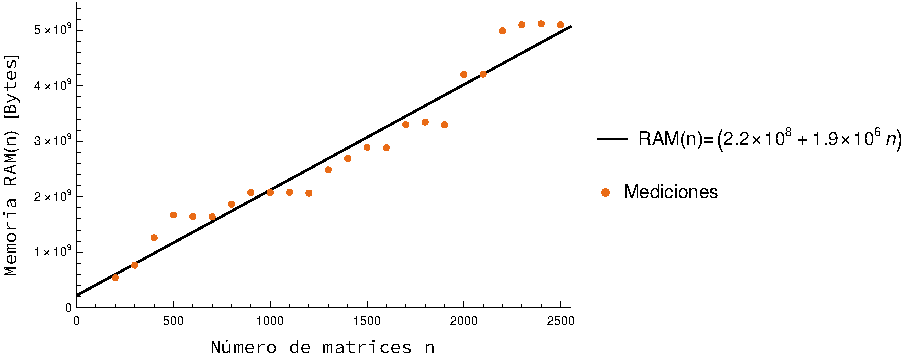
\includegraphics[width=\textwidth]{memory_usage_3Q_5c}
  \caption{Memoria RAM utilizada por el método numérico para analizar las
  operaciones PCE de 3 qubits que dejan invariantes 5 componentes de Pauli.
  El método numérico fue ejecutado en Wolfram Mathematica 12.1, operando
  en una PC con procesador Intel® Xeon(R) E-2246G~@~3.60GHz×12 
  y sistema operativo Ubuntu 20.04.3 LTS. \ep}
  \label{fig:memory_usage_3Q_5c}
\end{figure}

%\noindent
%\esqueleto{Con nuestro método numérico de fuerza bruta es posible 
%resolver el caso de 3 qubits hasta 4 componentes invariantes. Los resultados   
%son.... «con 3 qubits está todavía más jalado inferir características de 
%los canales PCE a partir de los 1's y 0's»}

Un subconjunto de todos los canales cuánticos PCE de 3 qubits, que encontramos 
de estudiar las operaciones PCE que dejan invariantes 1, 2, 3, 4, 61, 62, 63 y 64 
componentes de Pauli, los mostramos en la 
\Tref{tab:3qubitsPCEChannel1sAnd0s}. En total encontramos 716 canales cuánticos.
También encontramos que no hay canales PCE que dejen 
invariantes 3, 61, 62 o 63 componentes de Pauli. 
Adicional a estas dos observaciones, analizar las listas de 1's y 0's 
es todavía más enrevesado que las de los canales PCE de 2 qubits en la
\Tref{tab:2qubitsPCEChannel1sAnd0s}.
Con estos resultados de 3 qubits es indiscutible la necesidad de 
una herramienta geométrica para visualizar las listas 
de 1's y 0's de las operaciones PCE.

%Colocar en la \Tref{tab:3qubitsPCEChannel1sAnd0s}
%los 716 canales haría que la tabla ocupe algunas páginas y, al igual que para 2 
%qubits o incluso peor, las listas de 1's y 0''s así crudas aportan poco para el análisis 
%de las características que comparten los canales PCE. 

\janote{Comentario sobre la \Tref{tab:3qubitsPCEChannel1sAnd0s}: te parece necesario 
que ponga los casi 720 canales de 3 qubits que decimos aquí que pudimos
encontrar? Pregunto porque son como 10 páginas de tablas y me tomaría como 
1 hora dejarlas bonitas. Si no las ponemos, se dice que en el repositorio
que citamos en el capítulo anterior están los resultados. Sin embargo, también 
pienso que por el tipo de trabajo (una tesis) los resultados, así sean cochinamente largos,
deberían de poderse revisar aquí mismo en el manuscrito. 
Considera que en la siguiente sección que introduzco los tableritos no pretendo 
hacer una lista de figuras de todos los canales PCE de 3 qubits, cuando mucho 
sólo elementos representativos de familias de equivalencia.
Tú qué dices?}
 
\begin{landscape}
\begin{table}[]
\centering
\resizebox{0.82\paperheight}{!}{%
\begin{tabular}{|c|c|c|c|c|c|c|c|c|c|c|c|c|c|c|c|c|c|c|c|c|c|c|c|c|c|c|c|c|c|c|c|c|c|c|c|c|c|c|c|c|c|c|c|c|c|c|c|c|c|c|c|c|c|c|c|c|c|c|c|c|c|c|c|c|P{2.5cm}|}
\hline
\bf{No.} & \tauijk{0}{0}{0} & \tauijk{0}{0}{1} & \tauijk{0}{0}{2} & \tauijk{0}{0}{3} & \tauijk{0}{1}{0} & \tauijk{0}{1}{1} & \tauijk{0}{1}{2} & \tauijk{0}{1}{3} & \tauijk{0}{2}{0} & \tauijk{0}{2}{1} & \tauijk{0}{2}{2} & \tauijk{0}{2}{3} & \tauijk{0}{3}{0} & \tauijk{0}{3}{1} & \tauijk{0}{3}{2} & \tauijk{0}{3}{3} & \tauijk{1}{0}{0} & \tauijk{1}{0}{1} & \tauijk{1}{0}{2} & \tauijk{1}{0}{3} & \tauijk{1}{1}{0} & \tauijk{1}{1}{1} & \tauijk{1}{1}{2} & \tauijk{1}{1}{3} & \tauijk{1}{2}{0} & \tauijk{1}{2}{1} & \tauijk{1}{2}{2} & \tauijk{1}{2}{3} & \tauijk{1}{3}{0} & \tauijk{1}{3}{1} & \tauijk{1}{3}{2} & \tauijk{1}{3}{3} & \tauijk{2}{0}{0} & \tauijk{2}{0}{1} & \tauijk{2}{0}{2} & \tauijk{2}{0}{3} & \tauijk{2}{1}{0} & \tauijk{2}{1}{1} & \tauijk{2}{1}{2} & \tauijk{2}{1}{3} & \tauijk{2}{2}{0} & \tauijk{2}{2}{1} & \tauijk{2}{2}{2} & \tauijk{2}{2}{3} & \tauijk{2}{3}{0} & \tauijk{2}{3}{1} & \tauijk{2}{3}{2} & \tauijk{2}{3}{3} & \tauijk{3}{0}{0} & \tauijk{3}{0}{1} & \tauijk{3}{0}{2} & \tauijk{3}{0}{3} & \tauijk{3}{1}{0} & \tauijk{3}{1}{1} & \tauijk{3}{1}{2} & \tauijk{3}{1}{3} & \tauijk{3}{2}{0} & \tauijk{3}{2}{1} & \tauijk{3}{2}{2} & \tauijk{3}{2}{3} & \tauijk{3}{3}{0} & \tauijk{3}{3}{1} & \tauijk{3}{3}{2} & \tauijk{3}{3}{3} & \bf{Cantidad de \boldmath{$r_{ijk}$} invariantes} \\
\hline
\textbf{1}  & 1 & 1 & 1 & 1 & 0 & 0 & 0 & 0 & 0 & 0 & 0 & 0 & 0 & 0 & 0 & 0 & 0 & 0 & 0 & 0 & 0 & 0 & 0 & 0 & 0 & 0 & 0 & 0 & 0 & 0 & 0 & 0 & 0 & 0 & 0 & 0 & 0 & 0 & 0 & 0 & 0 & 0 & 0 & 0 & 0 & 0 & 0 & 0 & 0 & 0 & 0 & 0 & 0 & 0 & 0 & 0 & 0 & 0 & 0 & 0 & 0 & 0 & 0 & 0 \\
\hline
\textbf{2}  & 1 & 1 & 0 & 0 & 1 & 1 & 0 & 0 & 0 & 0 & 0 & 0 & 0 & 0 & 0 & 0 & 0 & 0 & 0 & 0 & 0 & 0 & 0 & 0 & 0 & 0 & 0 & 0 & 0 & 0 & 0 & 0 & 0 & 0 & 0 & 0 & 0 & 0 & 0 & 0 & 0 & 0 & 0 & 0 & 0 & 0 & 0 & 0 & 0 & 0 & 0 & 0 & 0 & 0 & 0 & 0 & 0 & 0 & 0 & 0 & 0 & 0 & 0 & 0 \\
\hline
\textbf{3}  & 1 & 1 & 0 & 0 & 0 & 0 & 1 & 1 & 0 & 0 & 0 & 0 & 0 & 0 & 0 & 0 & 0 & 0 & 0 & 0 & 0 & 0 & 0 & 0 & 0 & 0 & 0 & 0 & 0 & 0 & 0 & 0 & 0 & 0 & 0 & 0 & 0 & 0 & 0 & 0 & 0 & 0 & 0 & 0 & 0 & 0 & 0 & 0 & 0 & 0 & 0 & 0 & 0 & 0 & 0 & 0 & 0 & 0 & 0 & 0 & 0 & 0 & 0 & 0 \\
\hline
\textbf{4}  & 1 & 1 & 0 & 0 & 0 & 0 & 0 & 0 & 1 & 1 & 0 & 0 & 0 & 0 & 0 & 0 & 0 & 0 & 0 & 0 & 0 & 0 & 0 & 0 & 0 & 0 & 0 & 0 & 0 & 0 & 0 & 0 & 0 & 0 & 0 & 0 & 0 & 0 & 0 & 0 & 0 & 0 & 0 & 0 & 0 & 0 & 0 & 0 & 0 & 0 & 0 & 0 & 0 & 0 & 0 & 0 & 0 & 0 & 0 & 0 & 0 & 0 & 0 & 0 \\
\hline
\textbf{5}  & 1 & 1 & 0 & 0 & 0 & 0 & 0 & 0 & 0 & 0 & 1 & 1 & 0 & 0 & 0 & 0 & 0 & 0 & 0 & 0 & 0 & 0 & 0 & 0 & 0 & 0 & 0 & 0 & 0 & 0 & 0 & 0 & 0 & 0 & 0 & 0 & 0 & 0 & 0 & 0 & 0 & 0 & 0 & 0 & 0 & 0 & 0 & 0 & 0 & 0 & 0 & 0 & 0 & 0 & 0 & 0 & 0 & 0 & 0 & 0 & 0 & 0 & 0 & 0 \\
\hline
\textbf{6}  & 1 & 1 & 0 & 0 & 0 & 0 & 0 & 0 & 0 & 0 & 0 & 0 & 1 & 1 & 0 & 0 & 0 & 0 & 0 & 0 & 0 & 0 & 0 & 0 & 0 & 0 & 0 & 0 & 0 & 0 & 0 & 0 & 0 & 0 & 0 & 0 & 0 & 0 & 0 & 0 & 0 & 0 & 0 & 0 & 0 & 0 & 0 & 0 & 0 & 0 & 0 & 0 & 0 & 0 & 0 & 0 & 0 & 0 & 0 & 0 & 0 & 0 & 0 & 0 \\
\hline
\textbf{7}  & 1 & 1 & 0 & 0 & 0 & 0 & 0 & 0 & 0 & 0 & 0 & 0 & 0 & 0 & 1 & 1 & 0 & 0 & 0 & 0 & 0 & 0 & 0 & 0 & 0 & 0 & 0 & 0 & 0 & 0 & 0 & 0 & 0 & 0 & 0 & 0 & 0 & 0 & 0 & 0 & 0 & 0 & 0 & 0 & 0 & 0 & 0 & 0 & 0 & 0 & 0 & 0 & 0 & 0 & 0 & 0 & 0 & 0 & 0 & 0 & 0 & 0 & 0 & 0 \\
\hline
\textbf{8}  & 1 & 1 & 0 & 0 & 0 & 0 & 0 & 0 & 0 & 0 & 0 & 0 & 0 & 0 & 0 & 0 & 1 & 1 & 0 & 0 & 0 & 0 & 0 & 0 & 0 & 0 & 0 & 0 & 0 & 0 & 0 & 0 & 0 & 0 & 0 & 0 & 0 & 0 & 0 & 0 & 0 & 0 & 0 & 0 & 0 & 0 & 0 & 0 & 0 & 0 & 0 & 0 & 0 & 0 & 0 & 0 & 0 & 0 & 0 & 0 & 0 & 0 & 0 & 0 \\
\hline
\textbf{9}  & 1 & 1 & 0 & 0 & 0 & 0 & 0 & 0 & 0 & 0 & 0 & 0 & 0 & 0 & 0 & 0 & 0 & 0 & 1 & 1 & 0 & 0 & 0 & 0 & 0 & 0 & 0 & 0 & 0 & 0 & 0 & 0 & 0 & 0 & 0 & 0 & 0 & 0 & 0 & 0 & 0 & 0 & 0 & 0 & 0 & 0 & 0 & 0 & 0 & 0 & 0 & 0 & 0 & 0 & 0 & 0 & 0 & 0 & 0 & 0 & 0 & 0 & 0 & 0 \\
\hline
\textbf{10} & 1 & 1 & 0 & 0 & 0 & 0 & 0 & 0 & 0 & 0 & 0 & 0 & 0 & 0 & 0 & 0 & 0 & 0 & 0 & 0 & 1 & 1 & 0 & 0 & 0 & 0 & 0 & 0 & 0 & 0 & 0 & 0 & 0 & 0 & 0 & 0 & 0 & 0 & 0 & 0 & 0 & 0 & 0 & 0 & 0 & 0 & 0 & 0 & 0 & 0 & 0 & 0 & 0 & 0 & 0 & 0 & 0 & 0 & 0 & 0 & 0 & 0 & 0 & 0 \\
\hline
\textbf{11} & 1 & 1 & 0 & 0 & 0 & 0 & 0 & 0 & 0 & 0 & 0 & 0 & 0 & 0 & 0 & 0 & 0 & 0 & 0 & 0 & 0 & 0 & 1 & 1 & 0 & 0 & 0 & 0 & 0 & 0 & 0 & 0 & 0 & 0 & 0 & 0 & 0 & 0 & 0 & 0 & 0 & 0 & 0 & 0 & 0 & 0 & 0 & 0 & 0 & 0 & 0 & 0 & 0 & 0 & 0 & 0 & 0 & 0 & 0 & 0 & 0 & 0 & 0 & 0 \\
\hline
\textbf{12} & 1 & 1 & 0 & 0 & 0 & 0 & 0 & 0 & 0 & 0 & 0 & 0 & 0 & 0 & 0 & 0 & 0 & 0 & 0 & 0 & 0 & 0 & 0 & 0 & 1 & 1 & 0 & 0 & 0 & 0 & 0 & 0 & 0 & 0 & 0 & 0 & 0 & 0 & 0 & 0 & 0 & 0 & 0 & 0 & 0 & 0 & 0 & 0 & 0 & 0 & 0 & 0 & 0 & 0 & 0 & 0 & 0 & 0 & 0 & 0 & 0 & 0 & 0 & 0 \\
\hline
\textbf{13} & 1 & 1 & 0 & 0 & 0 & 0 & 0 & 0 & 0 & 0 & 0 & 0 & 0 & 0 & 0 & 0 & 0 & 0 & 0 & 0 & 0 & 0 & 0 & 0 & 0 & 0 & 1 & 1 & 0 & 0 & 0 & 0 & 0 & 0 & 0 & 0 & 0 & 0 & 0 & 0 & 0 & 0 & 0 & 0 & 0 & 0 & 0 & 0 & 0 & 0 & 0 & 0 & 0 & 0 & 0 & 0 & 0 & 0 & 0 & 0 & 0 & 0 & 0 & 0 \\
\hline
\textbf{14} & 1 & 1 & 0 & 0 & 0 & 0 & 0 & 0 & 0 & 0 & 0 & 0 & 0 & 0 & 0 & 0 & 0 & 0 & 0 & 0 & 0 & 0 & 0 & 0 & 0 & 0 & 0 & 0 & 1 & 1 & 0 & 0 & 0 & 0 & 0 & 0 & 0 & 0 & 0 & 0 & 0 & 0 & 0 & 0 & 0 & 0 & 0 & 0 & 0 & 0 & 0 & 0 & 0 & 0 & 0 & 0 & 0 & 0 & 0 & 0 & 0 & 0 & 0 & 0 \\
\hline
\textbf{15} & 1 & 1 & 0 & 0 & 0 & 0 & 0 & 0 & 0 & 0 & 0 & 0 & 0 & 0 & 0 & 0 & 0 & 0 & 0 & 0 & 0 & 0 & 0 & 0 & 0 & 0 & 0 & 0 & 0 & 0 & 1 & 1 & 0 & 0 & 0 & 0 & 0 & 0 & 0 & 0 & 0 & 0 & 0 & 0 & 0 & 0 & 0 & 0 & 0 & 0 & 0 & 0 & 0 & 0 & 0 & 0 & 0 & 0 & 0 & 0 & 0 & 0 & 0 & 0 \\
\hline
\textbf{16} & 1 & 1 & 0 & 0 & 0 & 0 & 0 & 0 & 0 & 0 & 0 & 0 & 0 & 0 & 0 & 0 & 0 & 0 & 0 & 0 & 0 & 0 & 0 & 0 & 0 & 0 & 0 & 0 & 0 & 0 & 0 & 0 & 1 & 1 & 0 & 0 & 0 & 0 & 0 & 0 & 0 & 0 & 0 & 0 & 0 & 0 & 0 & 0 & 0 & 0 & 0 & 0 & 0 & 0 & 0 & 0 & 0 & 0 & 0 & 0 & 0 & 0 & 0 & 0 \\
\hline
\textbf{17} & 1 & 1 & 0 & 0 & 0 & 0 & 0 & 0 & 0 & 0 & 0 & 0 & 0 & 0 & 0 & 0 & 0 & 0 & 0 & 0 & 0 & 0 & 0 & 0 & 0 & 0 & 0 & 0 & 0 & 0 & 0 & 0 & 0 & 0 & 1 & 1 & 0 & 0 & 0 & 0 & 0 & 0 & 0 & 0 & 0 & 0 & 0 & 0 & 0 & 0 & 0 & 0 & 0 & 0 & 0 & 0 & 0 & 0 & 0 & 0 & 0 & 0 & 0 & 0 \\
\hline
\textbf{18} & 1 & 1 & 0 & 0 & 0 & 0 & 0 & 0 & 0 & 0 & 0 & 0 & 0 & 0 & 0 & 0 & 0 & 0 & 0 & 0 & 0 & 0 & 0 & 0 & 0 & 0 & 0 & 0 & 0 & 0 & 0 & 0 & 0 & 0 & 0 & 0 & 1 & 1 & 0 & 0 & 0 & 0 & 0 & 0 & 0 & 0 & 0 & 0 & 0 & 0 & 0 & 0 & 0 & 0 & 0 & 0 & 0 & 0 & 0 & 0 & 0 & 0 & 0 & 0 \\
\hline
\textbf{19} & 1 & 1 & 0 & 0 & 0 & 0 & 0 & 0 & 0 & 0 & 0 & 0 & 0 & 0 & 0 & 0 & 0 & 0 & 0 & 0 & 0 & 0 & 0 & 0 & 0 & 0 & 0 & 0 & 0 & 0 & 0 & 0 & 0 & 0 & 0 & 0 & 0 & 0 & 1 & 1 & 0 & 0 & 0 & 0 & 0 & 0 & 0 & 0 & 0 & 0 & 0 & 0 & 0 & 0 & 0 & 0 & 0 & 0 & 0 & 0 & 0 & 0 & 0 & 0 \\
\hline
\textbf{20} & 1 & 1 & 0 & 0 & 0 & 0 & 0 & 0 & 0 & 0 & 0 & 0 & 0 & 0 & 0 & 0 & 0 & 0 & 0 & 0 & 0 & 0 & 0 & 0 & 0 & 0 & 0 & 0 & 0 & 0 & 0 & 0 & 0 & 0 & 0 & 0 & 0 & 0 & 0 & 0 & 1 & 1 & 0 & 0 & 0 & 0 & 0 & 0 & 0 & 0 & 0 & 0 & 0 & 0 & 0 & 0 & 0 & 0 & 0 & 0 & 0 & 0 & 0 & 0 \\
\hline
\textbf{21} & 1 & 1 & 0 & 0 & 0 & 0 & 0 & 0 & 0 & 0 & 0 & 0 & 0 & 0 & 0 & 0 & 0 & 0 & 0 & 0 & 0 & 0 & 0 & 0 & 0 & 0 & 0 & 0 & 0 & 0 & 0 & 0 & 0 & 0 & 0 & 0 & 0 & 0 & 0 & 0 & 0 & 0 & 1 & 1 & 0 & 0 & 0 & 0 & 0 & 0 & 0 & 0 & 0 & 0 & 0 & 0 & 0 & 0 & 0 & 0 & 0 & 0 & 0 & 0 \\
\hline
\textbf{22} & 1 & 1 & 0 & 0 & 0 & 0 & 0 & 0 & 0 & 0 & 0 & 0 & 0 & 0 & 0 & 0 & 0 & 0 & 0 & 0 & 0 & 0 & 0 & 0 & 0 & 0 & 0 & 0 & 0 & 0 & 0 & 0 & 0 & 0 & 0 & 0 & 0 & 0 & 0 & 0 & 0 & 0 & 0 & 0 & 1 & 1 & 0 & 0 & 0 & 0 & 0 & 0 & 0 & 0 & 0 & 0 & 0 & 0 & 0 & 0 & 0 & 0 & 0 & 0 \\
\hline
\textbf{23} & 1 & 1 & 0 & 0 & 0 & 0 & 0 & 0 & 0 & 0 & 0 & 0 & 0 & 0 & 0 & 0 & 0 & 0 & 0 & 0 & 0 & 0 & 0 & 0 & 0 & 0 & 0 & 0 & 0 & 0 & 0 & 0 & 0 & 0 & 0 & 0 & 0 & 0 & 0 & 0 & 0 & 0 & 0 & 0 & 0 & 0 & 1 & 1 & 0 & 0 & 0 & 0 & 0 & 0 & 0 & 0 & 0 & 0 & 0 & 0 & 0 & 0 & 0 & 0 \\
\hline
\textbf{24} & 1 & 1 & 0 & 0 & 0 & 0 & 0 & 0 & 0 & 0 & 0 & 0 & 0 & 0 & 0 & 0 & 0 & 0 & 0 & 0 & 0 & 0 & 0 & 0 & 0 & 0 & 0 & 0 & 0 & 0 & 0 & 0 & 0 & 0 & 0 & 0 & 0 & 0 & 0 & 0 & 0 & 0 & 0 & 0 & 0 & 0 & 0 & 0 & 1 & 1 & 0 & 0 & 0 & 0 & 0 & 0 & 0 & 0 & 0 & 0 & 0 & 0 & 0 & 0 \\
\hline
\textbf{25} & 1 & 1 & 0 & 0 & 0 & 0 & 0 & 0 & 0 & 0 & 0 & 0 & 0 & 0 & 0 & 0 & 0 & 0 & 0 & 0 & 0 & 0 & 0 & 0 & 0 & 0 & 0 & 0 & 0 & 0 & 0 & 0 & 0 & 0 & 0 & 0 & 0 & 0 & 0 & 0 & 0 & 0 & 0 & 0 & 0 & 0 & 0 & 0 & 0 & 0 & 1 & 1 & 0 & 0 & 0 & 0 & 0 & 0 & 0 & 0 & 0 & 0 & 0 & 0 \\
\hline
\textbf{26} & 1 & 1 & 0 & 0 & 0 & 0 & 0 & 0 & 0 & 0 & 0 & 0 & 0 & 0 & 0 & 0 & 0 & 0 & 0 & 0 & 0 & 0 & 0 & 0 & 0 & 0 & 0 & 0 & 0 & 0 & 0 & 0 & 0 & 0 & 0 & 0 & 0 & 0 & 0 & 0 & 0 & 0 & 0 & 0 & 0 & 0 & 0 & 0 & 0 & 0 & 0 & 0 & 1 & 1 & 0 & 0 & 0 & 0 & 0 & 0 & 0 & 0 & 0 & 0 \\
\hline
\textbf{27} & 1 & 1 & 0 & 0 & 0 & 0 & 0 & 0 & 0 & 0 & 0 & 0 & 0 & 0 & 0 & 0 & 0 & 0 & 0 & 0 & 0 & 0 & 0 & 0 & 0 & 0 & 0 & 0 & 0 & 0 & 0 & 0 & 0 & 0 & 0 & 0 & 0 & 0 & 0 & 0 & 0 & 0 & 0 & 0 & 0 & 0 & 0 & 0 & 0 & 0 & 0 & 0 & 0 & 0 & 1 & 1 & 0 & 0 & 0 & 0 & 0 & 0 & 0 & 0 \\
\hline
\textbf{28} & 1 & 1 & 0 & 0 & 0 & 0 & 0 & 0 & 0 & 0 & 0 & 0 & 0 & 0 & 0 & 0 & 0 & 0 & 0 & 0 & 0 & 0 & 0 & 0 & 0 & 0 & 0 & 0 & 0 & 0 & 0 & 0 & 0 & 0 & 0 & 0 & 0 & 0 & 0 & 0 & 0 & 0 & 0 & 0 & 0 & 0 & 0 & 0 & 0 & 0 & 0 & 0 & 0 & 0 & 0 & 0 & 1 & 1 & 0 & 0 & 0 & 0 & 0 & 0 \\
\hline
\textbf{29} & 1 & 1 & 0 & 0 & 0 & 0 & 0 & 0 & 0 & 0 & 0 & 0 & 0 & 0 & 0 & 0 & 0 & 0 & 0 & 0 & 0 & 0 & 0 & 0 & 0 & 0 & 0 & 0 & 0 & 0 & 0 & 0 & 0 & 0 & 0 & 0 & 0 & 0 & 0 & 0 & 0 & 0 & 0 & 0 & 0 & 0 & 0 & 0 & 0 & 0 & 0 & 0 & 0 & 0 & 0 & 0 & 0 & 0 & 1 & 1 & 0 & 0 & 0 & 0 \\
\hline
\textbf{30} & 1 & 1 & 0 & 0 & 0 & 0 & 0 & 0 & 0 & 0 & 0 & 0 & 0 & 0 & 0 & 0 & 0 & 0 & 0 & 0 & 0 & 0 & 0 & 0 & 0 & 0 & 0 & 0 & 0 & 0 & 0 & 0 & 0 & 0 & 0 & 0 & 0 & 0 & 0 & 0 & 0 & 0 & 0 & 0 & 0 & 0 & 0 & 0 & 0 & 0 & 0 & 0 & 0 & 0 & 0 & 0 & 0 & 0 & 0 & 0 & 1 & 1 & 0 & 0 \\
\hline
\textbf{31} & 1 & 1 & 0 & 0 & 0 & 0 & 0 & 0 & 0 & 0 & 0 & 0 & 0 & 0 & 0 & 0 & 0 & 0 & 0 & 0 & 0 & 0 & 0 & 0 & 0 & 0 & 0 & 0 & 0 & 0 & 0 & 0 & 0 & 0 & 0 & 0 & 0 & 0 & 0 & 0 & 0 & 0 & 0 & 0 & 0 & 0 & 0 & 0 & 0 & 0 & 0 & 0 & 0 & 0 & 0 & 0 & 0 & 0 & 0 & 0 & 0 & 0 & 1 & 1 \\
\hline
\textbf{32} & 1 & 0 & 1 & 0 & 1 & 0 & 1 & 0 & 0 & 0 & 0 & 0 & 0 & 0 & 0 & 0 & 0 & 0 & 0 & 0 & 0 & 0 & 0 & 0 & 0 & 0 & 0 & 0 & 0 & 0 & 0 & 0 & 0 & 0 & 0 & 0 & 0 & 0 & 0 & 0 & 0 & 0 & 0 & 0 & 0 & 0 & 0 & 0 & 0 & 0 & 0 & 0 & 0 & 0 & 0 & 0 & 0 & 0 & 0 & 0 & 0 & 0 & 0 & 0 \\
\hline
\textbf{33} & 1 & 0 & 1 & 0 & 0 & 1 & 0 & 1 & 0 & 0 & 0 & 0 & 0 & 0 & 0 & 0 & 0 & 0 & 0 & 0 & 0 & 0 & 0 & 0 & 0 & 0 & 0 & 0 & 0 & 0 & 0 & 0 & 0 & 0 & 0 & 0 & 0 & 0 & 0 & 0 & 0 & 0 & 0 & 0 & 0 & 0 & 0 & 0 & 0 & 0 & 0 & 0 & 0 & 0 & 0 & 0 & 0 & 0 & 0 & 0 & 0 & 0 & 0 & 0 \\
\hline
\textbf{34} & 1 & 0 & 1 & 0 & 0 & 0 & 0 & 0 & 1 & 0 & 1 & 0 & 0 & 0 & 0 & 0 & 0 & 0 & 0 & 0 & 0 & 0 & 0 & 0 & 0 & 0 & 0 & 0 & 0 & 0 & 0 & 0 & 0 & 0 & 0 & 0 & 0 & 0 & 0 & 0 & 0 & 0 & 0 & 0 & 0 & 0 & 0 & 0 & 0 & 0 & 0 & 0 & 0 & 0 & 0 & 0 & 0 & 0 & 0 & 0 & 0 & 0 & 0 & 0 \\
\hline
\textbf{35} & 1 & 0 & 1 & 0 & 0 & 0 & 0 & 0 & 0 & 1 & 0 & 1 & 0 & 0 & 0 & 0 & 0 & 0 & 0 & 0 & 0 & 0 & 0 & 0 & 0 & 0 & 0 & 0 & 0 & 0 & 0 & 0 & 0 & 0 & 0 & 0 & 0 & 0 & 0 & 0 & 0 & 0 & 0 & 0 & 0 & 0 & 0 & 0 & 0 & 0 & 0 & 0 & 0 & 0 & 0 & 0 & 0 & 0 & 0 & 0 & 0 & 0 & 0 & 0 \\
\hline
\textbf{36} & 1 & 0 & 1 & 0 & 0 & 0 & 0 & 0 & 0 & 0 & 0 & 0 & 1 & 0 & 1 & 0 & 0 & 0 & 0 & 0 & 0 & 0 & 0 & 0 & 0 & 0 & 0 & 0 & 0 & 0 & 0 & 0 & 0 & 0 & 0 & 0 & 0 & 0 & 0 & 0 & 0 & 0 & 0 & 0 & 0 & 0 & 0 & 0 & 0 & 0 & 0 & 0 & 0 & 0 & 0 & 0 & 0 & 0 & 0 & 0 & 0 & 0 & 0 & 0 \\
\hline
\textbf{37} & 1 & 0 & 1 & 0 & 0 & 0 & 0 & 0 & 0 & 0 & 0 & 0 & 0 & 1 & 0 & 1 & 0 & 0 & 0 & 0 & 0 & 0 & 0 & 0 & 0 & 0 & 0 & 0 & 0 & 0 & 0 & 0 & 0 & 0 & 0 & 0 & 0 & 0 & 0 & 0 & 0 & 0 & 0 & 0 & 0 & 0 & 0 & 0 & 0 & 0 & 0 & 0 & 0 & 0 & 0 & 0 & 0 & 0 & 0 & 0 & 0 & 0 & 0 & 0 \\
\hline
\textbf{38} & 1 & 0 & 1 & 0 & 0 & 0 & 0 & 0 & 0 & 0 & 0 & 0 & 0 & 0 & 0 & 0 & 1 & 0 & 1 & 0 & 0 & 0 & 0 & 0 & 0 & 0 & 0 & 0 & 0 & 0 & 0 & 0 & 0 & 0 & 0 & 0 & 0 & 0 & 0 & 0 & 0 & 0 & 0 & 0 & 0 & 0 & 0 & 0 & 0 & 0 & 0 & 0 & 0 & 0 & 0 & 0 & 0 & 0 & 0 & 0 & 0 & 0 & 0 & 0 \\
\hline
\textbf{39} & 1 & 0 & 1 & 0 & 0 & 0 & 0 & 0 & 0 & 0 & 0 & 0 & 0 & 0 & 0 & 0 & 0 & 1 & 0 & 1 & 0 & 0 & 0 & 0 & 0 & 0 & 0 & 0 & 0 & 0 & 0 & 0 & 0 & 0 & 0 & 0 & 0 & 0 & 0 & 0 & 0 & 0 & 0 & 0 & 0 & 0 & 0 & 0 & 0 & 0 & 0 & 0 & 0 & 0 & 0 & 0 & 0 & 0 & 0 & 0 & 0 & 0 & 0 & 0 \\
\hline
\textbf{40} & 1 & 0 & 1 & 0 & 0 & 0 & 0 & 0 & 0 & 0 & 0 & 0 & 0 & 0 & 0 & 0 & 0 & 0 & 0 & 0 & 1 & 0 & 1 & 0 & 0 & 0 & 0 & 0 & 0 & 0 & 0 & 0 & 0 & 0 & 0 & 0 & 0 & 0 & 0 & 0 & 0 & 0 & 0 & 0 & 0 & 0 & 0 & 0 & 0 & 0 & 0 & 0 & 0 & 0 & 0 & 0 & 0 & 0 & 0 & 0 & 0 & 0 & 0 & 0 \\
\hline
\textbf{41} & 1 & 0 & 1 & 0 & 0 & 0 & 0 & 0 & 0 & 0 & 0 & 0 & 0 & 0 & 0 & 0 & 0 & 0 & 0 & 0 & 0 & 1 & 0 & 1 & 0 & 0 & 0 & 0 & 0 & 0 & 0 & 0 & 0 & 0 & 0 & 0 & 0 & 0 & 0 & 0 & 0 & 0 & 0 & 0 & 0 & 0 & 0 & 0 & 0 & 0 & 0 & 0 & 0 & 0 & 0 & 0 & 0 & 0 & 0 & 0 & 0 & 0 & 0 & 0 \\
\hline
\textbf{42} & 1 & 0 & 1 & 0 & 0 & 0 & 0 & 0 & 0 & 0 & 0 & 0 & 0 & 0 & 0 & 0 & 0 & 0 & 0 & 0 & 0 & 0 & 0 & 0 & 1 & 0 & 1 & 0 & 0 & 0 & 0 & 0 & 0 & 0 & 0 & 0 & 0 & 0 & 0 & 0 & 0 & 0 & 0 & 0 & 0 & 0 & 0 & 0 & 0 & 0 & 0 & 0 & 0 & 0 & 0 & 0 & 0 & 0 & 0 & 0 & 0 & 0 & 0 & 0 \\
\hline
\textbf{43} & 1 & 0 & 1 & 0 & 0 & 0 & 0 & 0 & 0 & 0 & 0 & 0 & 0 & 0 & 0 & 0 & 0 & 0 & 0 & 0 & 0 & 0 & 0 & 0 & 0 & 1 & 0 & 1 & 0 & 0 & 0 & 0 & 0 & 0 & 0 & 0 & 0 & 0 & 0 & 0 & 0 & 0 & 0 & 0 & 0 & 0 & 0 & 0 & 0 & 0 & 0 & 0 & 0 & 0 & 0 & 0 & 0 & 0 & 0 & 0 & 0 & 0 & 0 & 0 \\
\hline
\textbf{44} & 1 & 0 & 1 & 0 & 0 & 0 & 0 & 0 & 0 & 0 & 0 & 0 & 0 & 0 & 0 & 0 & 0 & 0 & 0 & 0 & 0 & 0 & 0 & 0 & 0 & 0 & 0 & 0 & 1 & 0 & 1 & 0 & 0 & 0 & 0 & 0 & 0 & 0 & 0 & 0 & 0 & 0 & 0 & 0 & 0 & 0 & 0 & 0 & 0 & 0 & 0 & 0 & 0 & 0 & 0 & 0 & 0 & 0 & 0 & 0 & 0 & 0 & 0 & 0 \\
\hline
\textbf{45} & 1 & 0 & 1 & 0 & 0 & 0 & 0 & 0 & 0 & 0 & 0 & 0 & 0 & 0 & 0 & 0 & 0 & 0 & 0 & 0 & 0 & 0 & 0 & 0 & 0 & 0 & 0 & 0 & 0 & 1 & 0 & 1 & 0 & 0 & 0 & 0 & 0 & 0 & 0 & 0 & 0 & 0 & 0 & 0 & 0 & 0 & 0 & 0 & 0 & 0 & 0 & 0 & 0 & 0 & 0 & 0 & 0 & 0 & 0 & 0 & 0 & 0 & 0 & 0 \\
\hline
\textbf{46} & 1 & 0 & 1 & 0 & 0 & 0 & 0 & 0 & 0 & 0 & 0 & 0 & 0 & 0 & 0 & 0 & 0 & 0 & 0 & 0 & 0 & 0 & 0 & 0 & 0 & 0 & 0 & 0 & 0 & 0 & 0 & 0 & 1 & 0 & 1 & 0 & 0 & 0 & 0 & 0 & 0 & 0 & 0 & 0 & 0 & 0 & 0 & 0 & 0 & 0 & 0 & 0 & 0 & 0 & 0 & 0 & 0 & 0 & 0 & 0 & 0 & 0 & 0 & 0 \\
\hline
\textbf{47} & 1 & 0 & 1 & 0 & 0 & 0 & 0 & 0 & 0 & 0 & 0 & 0 & 0 & 0 & 0 & 0 & 0 & 0 & 0 & 0 & 0 & 0 & 0 & 0 & 0 & 0 & 0 & 0 & 0 & 0 & 0 & 0 & 0 & 1 & 0 & 1 & 0 & 0 & 0 & 0 & 0 & 0 & 0 & 0 & 0 & 0 & 0 & 0 & 0 & 0 & 0 & 0 & 0 & 0 & 0 & 0 & 0 & 0 & 0 & 0 & 0 & 0 & 0 & 0 \\
\hline
\textbf{48} & 1 & 0 & 1 & 0 & 0 & 0 & 0 & 0 & 0 & 0 & 0 & 0 & 0 & 0 & 0 & 0 & 0 & 0 & 0 & 0 & 0 & 0 & 0 & 0 & 0 & 0 & 0 & 0 & 0 & 0 & 0 & 0 & 0 & 0 & 0 & 0 & 1 & 0 & 1 & 0 & 0 & 0 & 0 & 0 & 0 & 0 & 0 & 0 & 0 & 0 & 0 & 0 & 0 & 0 & 0 & 0 & 0 & 0 & 0 & 0 & 0 & 0 & 0 & 0 \\
\hline
\textbf{49} & 1 & 0 & 1 & 0 & 0 & 0 & 0 & 0 & 0 & 0 & 0 & 0 & 0 & 0 & 0 & 0 & 0 & 0 & 0 & 0 & 0 & 0 & 0 & 0 & 0 & 0 & 0 & 0 & 0 & 0 & 0 & 0 & 0 & 0 & 0 & 0 & 0 & 1 & 0 & 1 & 0 & 0 & 0 & 0 & 0 & 0 & 0 & 0 & 0 & 0 & 0 & 0 & 0 & 0 & 0 & 0 & 0 & 0 & 0 & 0 & 0 & 0 & 0 & 0 \\
\hline
\textbf{50} & 1 & 0 & 1 & 0 & 0 & 0 & 0 & 0 & 0 & 0 & 0 & 0 & 0 & 0 & 0 & 0 & 0 & 0 & 0 & 0 & 0 & 0 & 0 & 0 & 0 & 0 & 0 & 0 & 0 & 0 & 0 & 0 & 0 & 0 & 0 & 0 & 0 & 0 & 0 & 0 & 1 & 0 & 1 & 0 & 0 & 0 & 0 & 0 & 0 & 0 & 0 & 0 & 0 & 0 & 0 & 0 & 0 & 0 & 0 & 0 & 0 & 0 & 0 & 0 \\
\hline
\textbf{51} & 1 & 0 & 1 & 0 & 0 & 0 & 0 & 0 & 0 & 0 & 0 & 0 & 0 & 0 & 0 & 0 & 0 & 0 & 0 & 0 & 0 & 0 & 0 & 0 & 0 & 0 & 0 & 0 & 0 & 0 & 0 & 0 & 0 & 0 & 0 & 0 & 0 & 0 & 0 & 0 & 0 & 1 & 0 & 1 & 0 & 0 & 0 & 0 & 0 & 0 & 0 & 0 & 0 & 0 & 0 & 0 & 0 & 0 & 0 & 0 & 0 & 0 & 0 & 0 \\
\hline
\textbf{52} & 1 & 0 & 1 & 0 & 0 & 0 & 0 & 0 & 0 & 0 & 0 & 0 & 0 & 0 & 0 & 0 & 0 & 0 & 0 & 0 & 0 & 0 & 0 & 0 & 0 & 0 & 0 & 0 & 0 & 0 & 0 & 0 & 0 & 0 & 0 & 0 & 0 & 0 & 0 & 0 & 0 & 0 & 0 & 0 & 1 & 0 & 1 & 0 & 0 & 0 & 0 & 0 & 0 & 0 & 0 & 0 & 0 & 0 & 0 & 0 & 0 & 0 & 0 & 0 \\
\hline
\textbf{53} & 1 & 0 & 1 & 0 & 0 & 0 & 0 & 0 & 0 & 0 & 0 & 0 & 0 & 0 & 0 & 0 & 0 & 0 & 0 & 0 & 0 & 0 & 0 & 0 & 0 & 0 & 0 & 0 & 0 & 0 & 0 & 0 & 0 & 0 & 0 & 0 & 0 & 0 & 0 & 0 & 0 & 0 & 0 & 0 & 0 & 1 & 0 & 1 & 0 & 0 & 0 & 0 & 0 & 0 & 0 & 0 & 0 & 0 & 0 & 0 & 0 & 0 & 0 & 0 \\
\hline
\textbf{54} & 1 & 0 & 1 & 0 & 0 & 0 & 0 & 0 & 0 & 0 & 0 & 0 & 0 & 0 & 0 & 0 & 0 & 0 & 0 & 0 & 0 & 0 & 0 & 0 & 0 & 0 & 0 & 0 & 0 & 0 & 0 & 0 & 0 & 0 & 0 & 0 & 0 & 0 & 0 & 0 & 0 & 0 & 0 & 0 & 0 & 0 & 0 & 0 & 1 & 0 & 1 & 0 & 0 & 0 & 0 & 0 & 0 & 0 & 0 & 0 & 0 & 0 & 0 & 0 \\
\hline
\textbf{55} & 1 & 0 & 1 & 0 & 0 & 0 & 0 & 0 & 0 & 0 & 0 & 0 & 0 & 0 & 0 & 0 & 0 & 0 & 0 & 0 & 0 & 0 & 0 & 0 & 0 & 0 & 0 & 0 & 0 & 0 & 0 & 0 & 0 & 0 & 0 & 0 & 0 & 0 & 0 & 0 & 0 & 0 & 0 & 0 & 0 & 0 & 0 & 0 & 0 & 1 & 0 & 1 & 0 & 0 & 0 & 0 & 0 & 0 & 0 & 0 & 0 & 0 & 0 & 0 \\
\hline
\textbf{56} & 1 & 0 & 1 & 0 & 0 & 0 & 0 & 0 & 0 & 0 & 0 & 0 & 0 & 0 & 0 & 0 & 0 & 0 & 0 & 0 & 0 & 0 & 0 & 0 & 0 & 0 & 0 & 0 & 0 & 0 & 0 & 0 & 0 & 0 & 0 & 0 & 0 & 0 & 0 & 0 & 0 & 0 & 0 & 0 & 0 & 0 & 0 & 0 & 0 & 0 & 0 & 0 & 1 & 0 & 1 & 0 & 0 & 0 & 0 & 0 & 0 & 0 & 0 & 0 \\
\hline
\textbf{57} & 1 & 0 & 1 & 0 & 0 & 0 & 0 & 0 & 0 & 0 & 0 & 0 & 0 & 0 & 0 & 0 & 0 & 0 & 0 & 0 & 0 & 0 & 0 & 0 & 0 & 0 & 0 & 0 & 0 & 0 & 0 & 0 & 0 & 0 & 0 & 0 & 0 & 0 & 0 & 0 & 0 & 0 & 0 & 0 & 0 & 0 & 0 & 0 & 0 & 0 & 0 & 0 & 0 & 1 & 0 & 1 & 0 & 0 & 0 & 0 & 0 & 0 & 0 & 0 \\
\hline
\textbf{58} & 1 & 0 & 1 & 0 & 0 & 0 & 0 & 0 & 0 & 0 & 0 & 0 & 0 & 0 & 0 & 0 & 0 & 0 & 0 & 0 & 0 & 0 & 0 & 0 & 0 & 0 & 0 & 0 & 0 & 0 & 0 & 0 & 0 & 0 & 0 & 0 & 0 & 0 & 0 & 0 & 0 & 0 & 0 & 0 & 0 & 0 & 0 & 0 & 0 & 0 & 0 & 0 & 0 & 0 & 0 & 0 & 1 & 0 & 1 & 0 & 0 & 0 & 0 & 0 \\
\hline
\textbf{59} & 1 & 0 & 1 & 0 & 0 & 0 & 0 & 0 & 0 & 0 & 0 & 0 & 0 & 0 & 0 & 0 & 0 & 0 & 0 & 0 & 0 & 0 & 0 & 0 & 0 & 0 & 0 & 0 & 0 & 0 & 0 & 0 & 0 & 0 & 0 & 0 & 0 & 0 & 0 & 0 & 0 & 0 & 0 & 0 & 0 & 0 & 0 & 0 & 0 & 0 & 0 & 0 & 0 & 0 & 0 & 0 & 0 & 1 & 0 & 1 & 0 & 0 & 0 & 0 \\
\hline
\textbf{60} & 1 & 0 & 1 & 0 & 0 & 0 & 0 & 0 & 0 & 0 & 0 & 0 & 0 & 0 & 0 & 0 & 0 & 0 & 0 & 0 & 0 & 0 & 0 & 0 & 0 & 0 & 0 & 0 & 0 & 0 & 0 & 0 & 0 & 0 & 0 & 0 & 0 & 0 & 0 & 0 & 0 & 0 & 0 & 0 & 0 & 0 & 0 & 0 & 0 & 0 & 0 & 0 & 0 & 0 & 0 & 0 & 0 & 0 & 0 & 0 & 1 & 0 & 1 & 0 \\
\hline
\textbf{61} & 1 & 0 & 1 & 0 & 0 & 0 & 0 & 0 & 0 & 0 & 0 & 0 & 0 & 0 & 0 & 0 & 0 & 0 & 0 & 0 & 0 & 0 & 0 & 0 & 0 & 0 & 0 & 0 & 0 & 0 & 0 & 0 & 0 & 0 & 0 & 0 & 0 & 0 & 0 & 0 & 0 & 0 & 0 & 0 & 0 & 0 & 0 & 0 & 0 & 0 & 0 & 0 & 0 & 0 & 0 & 0 & 0 & 0 & 0 & 0 & 0 & 1 & 0 & 1 \\
\hline
\textbf{62} & 1 & 0 & 0 & 1 & 1 & 0 & 0 & 1 & 0 & 0 & 0 & 0 & 0 & 0 & 0 & 0 & 0 & 0 & 0 & 0 & 0 & 0 & 0 & 0 & 0 & 0 & 0 & 0 & 0 & 0 & 0 & 0 & 0 & 0 & 0 & 0 & 0 & 0 & 0 & 0 & 0 & 0 & 0 & 0 & 0 & 0 & 0 & 0 & 0 & 0 & 0 & 0 & 0 & 0 & 0 & 0 & 0 & 0 & 0 & 0 & 0 & 0 & 0 & 0 \\
\hline
\textbf{63} & 1 & 0 & 0 & 1 & 0 & 1 & 1 & 0 & 0 & 0 & 0 & 0 & 0 & 0 & 0 & 0 & 0 & 0 & 0 & 0 & 0 & 0 & 0 & 0 & 0 & 0 & 0 & 0 & 0 & 0 & 0 & 0 & 0 & 0 & 0 & 0 & 0 & 0 & 0 & 0 & 0 & 0 & 0 & 0 & 0 & 0 & 0 & 0 & 0 & 0 & 0 & 0 & 0 & 0 & 0 & 0 & 0 & 0 & 0 & 0 & 0 & 0 & 0 & 0 \\
\hline
\textbf{64} & 1 & 0 & 0 & 1 & 0 & 0 & 0 & 0 & 1 & 0 & 0 & 1 & 0 & 0 & 0 & 0 & 0 & 0 & 0 & 0 & 0 & 0 & 0 & 0 & 0 & 0 & 0 & 0 & 0 & 0 & 0 & 0 & 0 & 0 & 0 & 0 & 0 & 0 & 0 & 0 & 0 & 0 & 0 & 0 & 0 & 0 & 0 & 0 & 0 & 0 & 0 & 0 & 0 & 0 & 0 & 0 & 0 & 0 & 0 & 0 & 0 & 0 & 0 & 0 \\
\hline
\textbf{65} & 1 & 0 & 0 & 1 & 0 & 0 & 0 & 0 & 0 & 1 & 1 & 0 & 0 & 0 & 0 & 0 & 0 & 0 & 0 & 0 & 0 & 0 & 0 & 0 & 0 & 0 & 0 & 0 & 0 & 0 & 0 & 0 & 0 & 0 & 0 & 0 & 0 & 0 & 0 & 0 & 0 & 0 & 0 & 0 & 0 & 0 & 0 & 0 & 0 & 0 & 0 & 0 & 0 & 0 & 0 & 0 & 0 & 0 & 0 & 0 & 0 & 0 & 0 & 0 \\
\hline
\textbf{66} & 1 & 0 & 0 & 1 & 0 & 0 & 0 & 0 & 0 & 0 & 0 & 0 & 1 & 0 & 0 & 1 & 0 & 0 & 0 & 0 & 0 & 0 & 0 & 0 & 0 & 0 & 0 & 0 & 0 & 0 & 0 & 0 & 0 & 0 & 0 & 0 & 0 & 0 & 0 & 0 & 0 & 0 & 0 & 0 & 0 & 0 & 0 & 0 & 0 & 0 & 0 & 0 & 0 & 0 & 0 & 0 & 0 & 0 & 0 & 0 & 0 & 0 & 0 & 0 \\
\hline
\textbf{67} & 1 & 0 & 0 & 1 & 0 & 0 & 0 & 0 & 0 & 0 & 0 & 0 & 0 & 1 & 1 & 0 & 0 & 0 & 0 & 0 & 0 & 0 & 0 & 0 & 0 & 0 & 0 & 0 & 0 & 0 & 0 & 0 & 0 & 0 & 0 & 0 & 0 & 0 & 0 & 0 & 0 & 0 & 0 & 0 & 0 & 0 & 0 & 0 & 0 & 0 & 0 & 0 & 0 & 0 & 0 & 0 & 0 & 0 & 0 & 0 & 0 & 0 & 0 & 0 \\
\hline
\textbf{68} & 1 & 0 & 0 & 1 & 0 & 0 & 0 & 0 & 0 & 0 & 0 & 0 & 0 & 0 & 0 & 0 & 1 & 0 & 0 & 1 & 0 & 0 & 0 & 0 & 0 & 0 & 0 & 0 & 0 & 0 & 0 & 0 & 0 & 0 & 0 & 0 & 0 & 0 & 0 & 0 & 0 & 0 & 0 & 0 & 0 & 0 & 0 & 0 & 0 & 0 & 0 & 0 & 0 & 0 & 0 & 0 & 0 & 0 & 0 & 0 & 0 & 0 & 0 & 0 \\
\hline
\textbf{69} & 1 & 0 & 0 & 1 & 0 & 0 & 0 & 0 & 0 & 0 & 0 & 0 & 0 & 0 & 0 & 0 & 0 & 1 & 1 & 0 & 0 & 0 & 0 & 0 & 0 & 0 & 0 & 0 & 0 & 0 & 0 & 0 & 0 & 0 & 0 & 0 & 0 & 0 & 0 & 0 & 0 & 0 & 0 & 0 & 0 & 0 & 0 & 0 & 0 & 0 & 0 & 0 & 0 & 0 & 0 & 0 & 0 & 0 & 0 & 0 & 0 & 0 & 0 & 0 \\
\hline
\textbf{70} & 1 & 0 & 0 & 1 & 0 & 0 & 0 & 0 & 0 & 0 & 0 & 0 & 0 & 0 & 0 & 0 & 0 & 0 & 0 & 0 & 1 & 0 & 0 & 1 & 0 & 0 & 0 & 0 & 0 & 0 & 0 & 0 & 0 & 0 & 0 & 0 & 0 & 0 & 0 & 0 & 0 & 0 & 0 & 0 & 0 & 0 & 0 & 0 & 0 & 0 & 0 & 0 & 0 & 0 & 0 & 0 & 0 & 0 & 0 & 0 & 0 & 0 & 0 & 0 \\
\hline 
\textbf{60} & 1 & 0 & 1 & 0 & 0 & 0 & 0 & 0 & 0 & 0 & 0 & 0 & 0 & 0 & 0 & 0 & 0 & 0 & 0 & 0 & 0 & 0 & 0 & 0 & 0 & 0 & 0 & 0 & 0 & 0 & 0 & 0 & 0 & 0 & 0 & 0 & 0 & 0 & 0 & 0 & 0 & 0 & 0 & 0 & 0 & 0 & 0 & 0 & 0 & 0 & 0 & 0 & 0 & 0 & 0 & 0 & 0 & 0 & 0 & 0 & 1 & 0 & 1 & 0 \\
\hline
\textbf{61} & 1 & 0 & 1 & 0 & 0 & 0 & 0 & 0 & 0 & 0 & 0 & 0 & 0 & 0 & 0 & 0 & 0 & 0 & 0 & 0 & 0 & 0 & 0 & 0 & 0 & 0 & 0 & 0 & 0 & 0 & 0 & 0 & 0 & 0 & 0 & 0 & 0 & 0 & 0 & 0 & 0 & 0 & 0 & 0 & 0 & 0 & 0 & 0 & 0 & 0 & 0 & 0 & 0 & 0 & 0 & 0 & 0 & 0 & 0 & 0 & 0 & 1 & 0 & 1 \\
\hline
\textbf{62} & 1 & 0 & 0 & 1 & 1 & 0 & 0 & 1 & 0 & 0 & 0 & 0 & 0 & 0 & 0 & 0 & 0 & 0 & 0 & 0 & 0 & 0 & 0 & 0 & 0 & 0 & 0 & 0 & 0 & 0 & 0 & 0 & 0 & 0 & 0 & 0 & 0 & 0 & 0 & 0 & 0 & 0 & 0 & 0 & 0 & 0 & 0 & 0 & 0 & 0 & 0 & 0 & 0 & 0 & 0 & 0 & 0 & 0 & 0 & 0 & 0 & 0 & 0 & 0 \\
\hline
\textbf{63} & 1 & 0 & 0 & 1 & 0 & 1 & 1 & 0 & 0 & 0 & 0 & 0 & 0 & 0 & 0 & 0 & 0 & 0 & 0 & 0 & 0 & 0 & 0 & 0 & 0 & 0 & 0 & 0 & 0 & 0 & 0 & 0 & 0 & 0 & 0 & 0 & 0 & 0 & 0 & 0 & 0 & 0 & 0 & 0 & 0 & 0 & 0 & 0 & 0 & 0 & 0 & 0 & 0 & 0 & 0 & 0 & 0 & 0 & 0 & 0 & 0 & 0 & 0 & 0 \\
\hline
\textbf{64} & 1 & 0 & 0 & 1 & 0 & 0 & 0 & 0 & 1 & 0 & 0 & 1 & 0 & 0 & 0 & 0 & 0 & 0 & 0 & 0 & 0 & 0 & 0 & 0 & 0 & 0 & 0 & 0 & 0 & 0 & 0 & 0 & 0 & 0 & 0 & 0 & 0 & 0 & 0 & 0 & 0 & 0 & 0 & 0 & 0 & 0 & 0 & 0 & 0 & 0 & 0 & 0 & 0 & 0 & 0 & 0 & 0 & 0 & 0 & 0 & 0 & 0 & 0 & 0 \\
\hline
\textbf{65} & 1 & 0 & 0 & 1 & 0 & 0 & 0 & 0 & 0 & 1 & 1 & 0 & 0 & 0 & 0 & 0 & 0 & 0 & 0 & 0 & 0 & 0 & 0 & 0 & 0 & 0 & 0 & 0 & 0 & 0 & 0 & 0 & 0 & 0 & 0 & 0 & 0 & 0 & 0 & 0 & 0 & 0 & 0 & 0 & 0 & 0 & 0 & 0 & 0 & 0 & 0 & 0 & 0 & 0 & 0 & 0 & 0 & 0 & 0 & 0 & 0 & 0 & 0 & 0 \\
\hline
\textbf{66} & 1 & 0 & 0 & 1 & 0 & 0 & 0 & 0 & 0 & 0 & 0 & 0 & 1 & 0 & 0 & 1 & 0 & 0 & 0 & 0 & 0 & 0 & 0 & 0 & 0 & 0 & 0 & 0 & 0 & 0 & 0 & 0 & 0 & 0 & 0 & 0 & 0 & 0 & 0 & 0 & 0 & 0 & 0 & 0 & 0 & 0 & 0 & 0 & 0 & 0 & 0 & 0 & 0 & 0 & 0 & 0 & 0 & 0 & 0 & 0 & 0 & 0 & 0 & 0 \\
\hline
\textbf{67} & 1 & 0 & 0 & 1 & 0 & 0 & 0 & 0 & 0 & 0 & 0 & 0 & 0 & 1 & 1 & 0 & 0 & 0 & 0 & 0 & 0 & 0 & 0 & 0 & 0 & 0 & 0 & 0 & 0 & 0 & 0 & 0 & 0 & 0 & 0 & 0 & 0 & 0 & 0 & 0 & 0 & 0 & 0 & 0 & 0 & 0 & 0 & 0 & 0 & 0 & 0 & 0 & 0 & 0 & 0 & 0 & 0 & 0 & 0 & 0 & 0 & 0 & 0 & 0 \\
\hline
\textbf{68} & 1 & 0 & 0 & 1 & 0 & 0 & 0 & 0 & 0 & 0 & 0 & 0 & 0 & 0 & 0 & 0 & 1 & 0 & 0 & 1 & 0 & 0 & 0 & 0 & 0 & 0 & 0 & 0 & 0 & 0 & 0 & 0 & 0 & 0 & 0 & 0 & 0 & 0 & 0 & 0 & 0 & 0 & 0 & 0 & 0 & 0 & 0 & 0 & 0 & 0 & 0 & 0 & 0 & 0 & 0 & 0 & 0 & 0 & 0 & 0 & 0 & 0 & 0 & 0 \\
\hline
\textbf{69} & 1 & 0 & 0 & 1 & 0 & 0 & 0 & 0 & 0 & 0 & 0 & 0 & 0 & 0 & 0 & 0 & 0 & 1 & 1 & 0 & 0 & 0 & 0 & 0 & 0 & 0 & 0 & 0 & 0 & 0 & 0 & 0 & 0 & 0 & 0 & 0 & 0 & 0 & 0 & 0 & 0 & 0 & 0 & 0 & 0 & 0 & 0 & 0 & 0 & 0 & 0 & 0 & 0 & 0 & 0 & 0 & 0 & 0 & 0 & 0 & 0 & 0 & 0 & 0 \\
\hline
\textbf{70} & 1 & 0 & 0 & 1 & 0 & 0 & 0 & 0 & 0 & 0 & 0 & 0 & 0 & 0 & 0 & 0 & 0 & 0 & 0 & 0 & 1 & 0 & 0 & 1 & 0 & 0 & 0 & 0 & 0 & 0 & 0 & 0 & 0 & 0 & 0 & 0 & 0 & 0 & 0 & 0 & 0 & 0 & 0 & 0 & 0 & 0 & 0 & 0 & 0 & 0 & 0 & 0 & 0 & 0 & 0 & 0 & 0 & 0 & 0 & 0 & 0 & 0 & 0 & 0 \\
\hline
\end{tabular}
}
\caption{Canales cuánticos PCE de 3 qubits.}
\label{tab:3qubitsPCEChannel1sAnd0s}
\end{table}
\end{landscape}

\section{Una representación geométrica}\label{sec:ch3_geometric_representation}
%\esqueleto{Motivados en lo intricado de inferir qué características 
%comparten los canales PCE a partir de las listas de 1's y 0's, se nos ocurrió 
%una forma de representar geométricamente a las operaciones PCE que hace
%más sencillo el análisis de resultados.}

En la sección anterior vimos que los resultados crudos, las listas de 1's y 0's 
de de los elementos $\taus$ de los canales PCE de 2 qubits y algunos de los 
de 3 qubits de las tablas \ref{tab:2qubitsPCEChannel1sAnd0s} y 
\ref{tab:3qubitsPCEChannel1sAnd0s}, no hacen sencilla la tarea de analizar 
las propiedades que comparten los canales cuánticos PCE. En vista de ello, 
buscamos una herramienta que nos permita visualizar y apreciar de una 
manera visual las características de un canal PCE, de manera similar que es 
la ayuda de la esfera de Bloch para 1 qubit.  Esta sección la dedicamos 
exclusivamente para introducir y discutir la herramienta de \janote{será 
que le ponemos nombre a esta onda?} para visualizar ''geométricamente``
a una operación PCE. 

%\esqueleto{La figura asociada con una operación PCE de 1 qubit 
%es una columna de 
%cuadritos.. bla bla y con figuritas, haciendo referencia a lo que se resolvió 
%en el capítulo anterior, etc.}

En la \Fref{fig:PCE_figs} introducimos las ``figuras PCE'' para representar 
a las operaciones PCE. Mostramos la figura PCE de la operación identidad
de 1, 2 y 3 qubits, una operación PCE con todos los elementos 
$\tau_i$, $\tau_{ij}$ y $\tau_{ijk}$, respectivamente, iguales a 1. En una 
figura PCE, la posición de cada cuadro o cubo está asociada con los índices 
$j_1,\ldots,j_n$ de los elementos $\taus$ de una operación PCE. Además, 
los cuadros pintados de color negro, en el caso de figuras PCE de 1 y 2 qubits, 
o cubos pintados de color rojo, azul o verde, en el caso de una figura PCE de 
3 qubits, están asociados con elementos $\tau_{k_1,\ldots,j_n}$ iguales a 1;
los cuadros o cubos no pintados están asociados con $\tau_{l_1,\ldots,l_n}$
iguales a 0. 
Los colores de las figuras PCE de 3 qubits no son más que una ayuda para visualizar 
mejor las operaciones PCE de 3 qubits. Los cubos con posiciones de la forma $(i,0,0)$,
$(0,j,0)$ y $(0,0,k)$ se pintan de rojo. Los cubos con posiciones de la forma $(i,j,0)$,
$(0,j,k)$ y $(i,0,k)$ se pintan de azul. Los cubos con posiciones de la forma $(i,j,k)$,
se pintan de verde. 
%\begin{figure} % {{{
%	\centering
%	\hfill \hfill
%	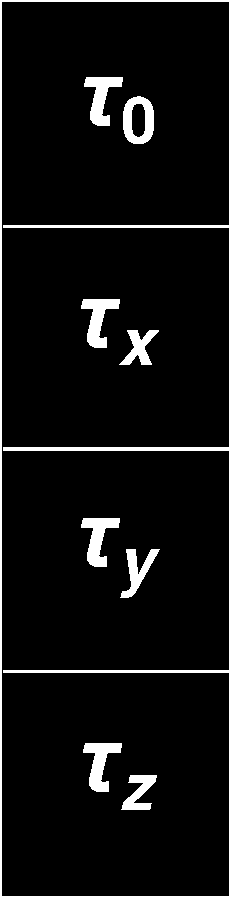
\includegraphics[height=3cm]	{tablero_1qubit}
%	\hspace{1.5cm}
%	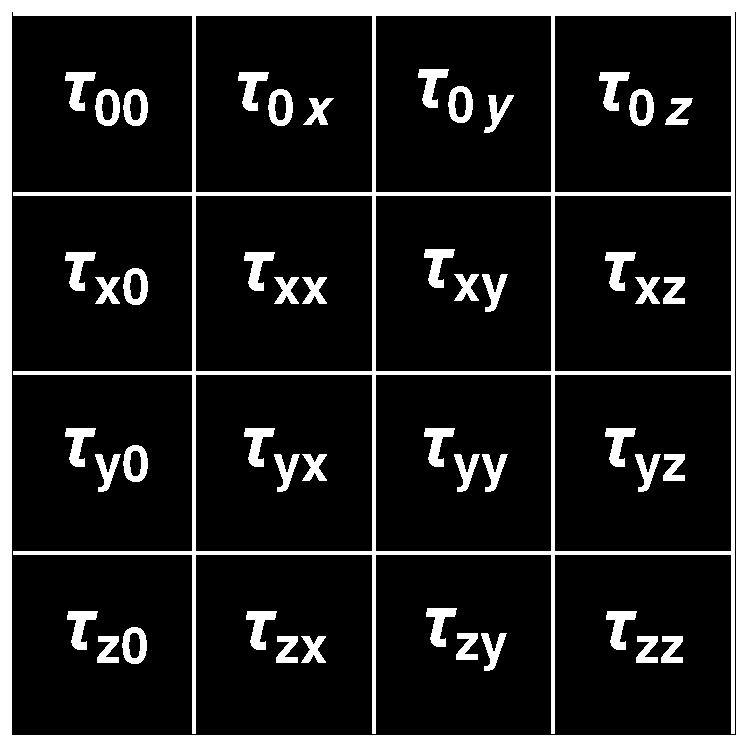
\includegraphics[height=3cm]{tablero_2qubits}
%	\hspace{.9cm}
%	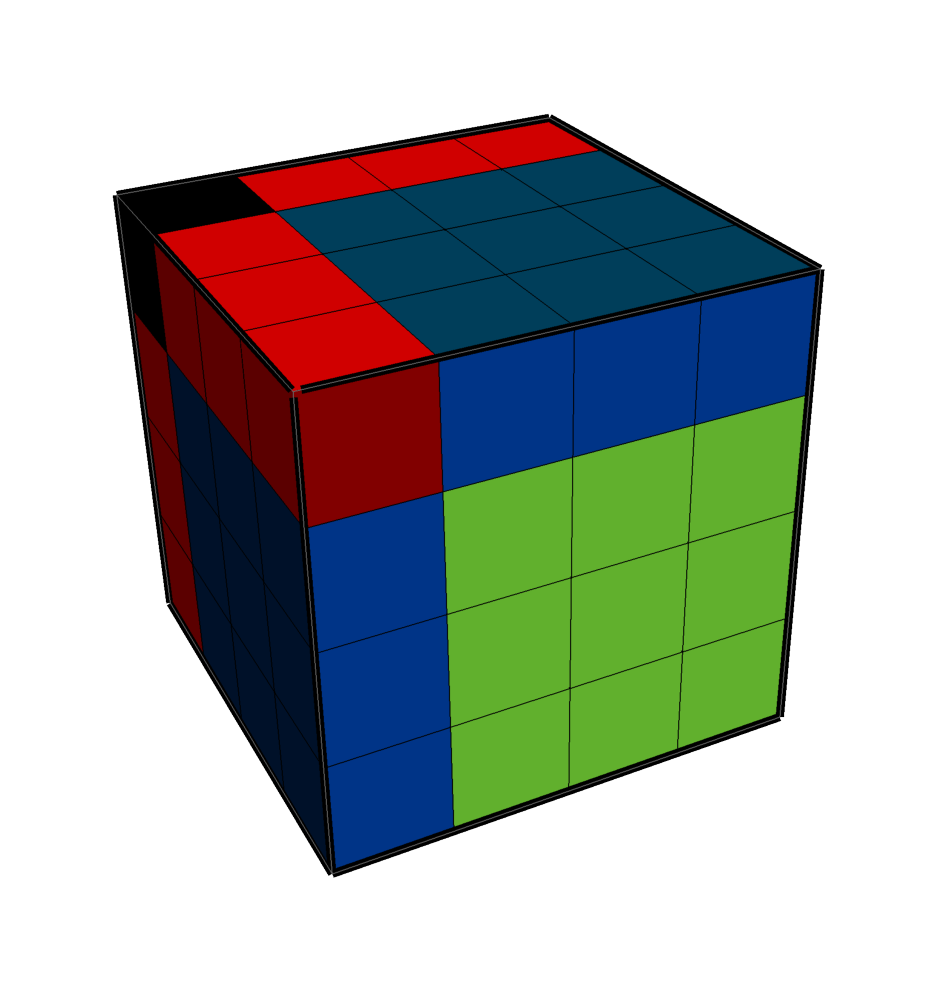
\includegraphics[height=3.3cm]{cubo_3qubits}
%	\hfill \hfill \hfill 
%	\caption{De izquierda a derecha se muestran la representación de la operación
%	identidad de 1, 2 y 3 qubits.  \ep}
%	\label{fig:PCE_figs}
%\end{figure} % }}}
\begin{figure} % {{{
	\centering
	\begin{subfigure}[b]{0.3\textwidth}
		\centering
		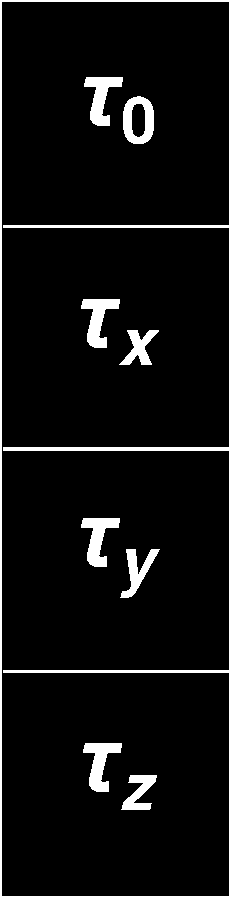
\includegraphics[height=3cm]	{tablero_1qubit}
		\caption{}
	\end{subfigure}
	\hfill
	\begin{subfigure}[b]{0.3\textwidth}
		\centering
		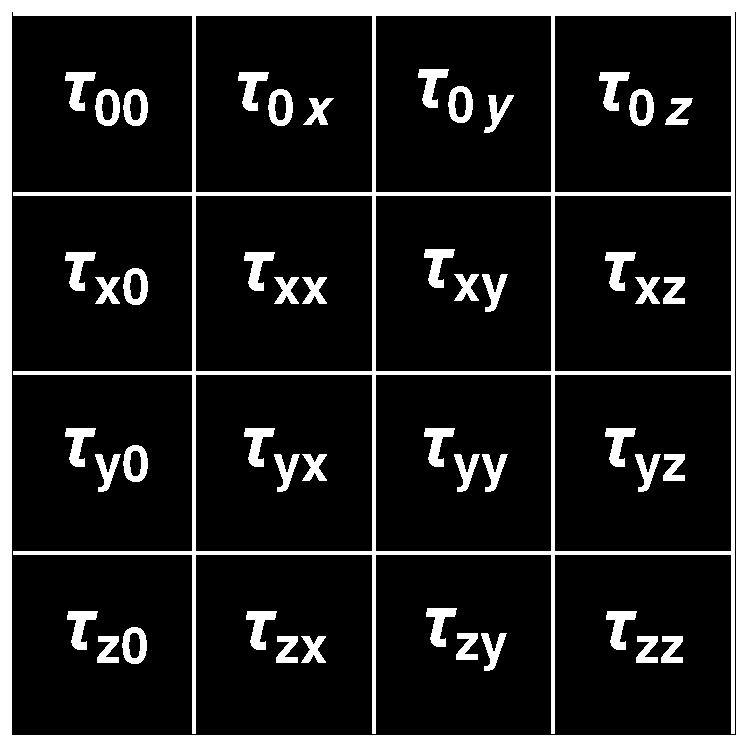
\includegraphics[height=3cm]{tablero_2qubits}
		\caption{}
	\end{subfigure}
	\hfill
	\begin{subfigure}[b]{0.3\textwidth}
		\centering
		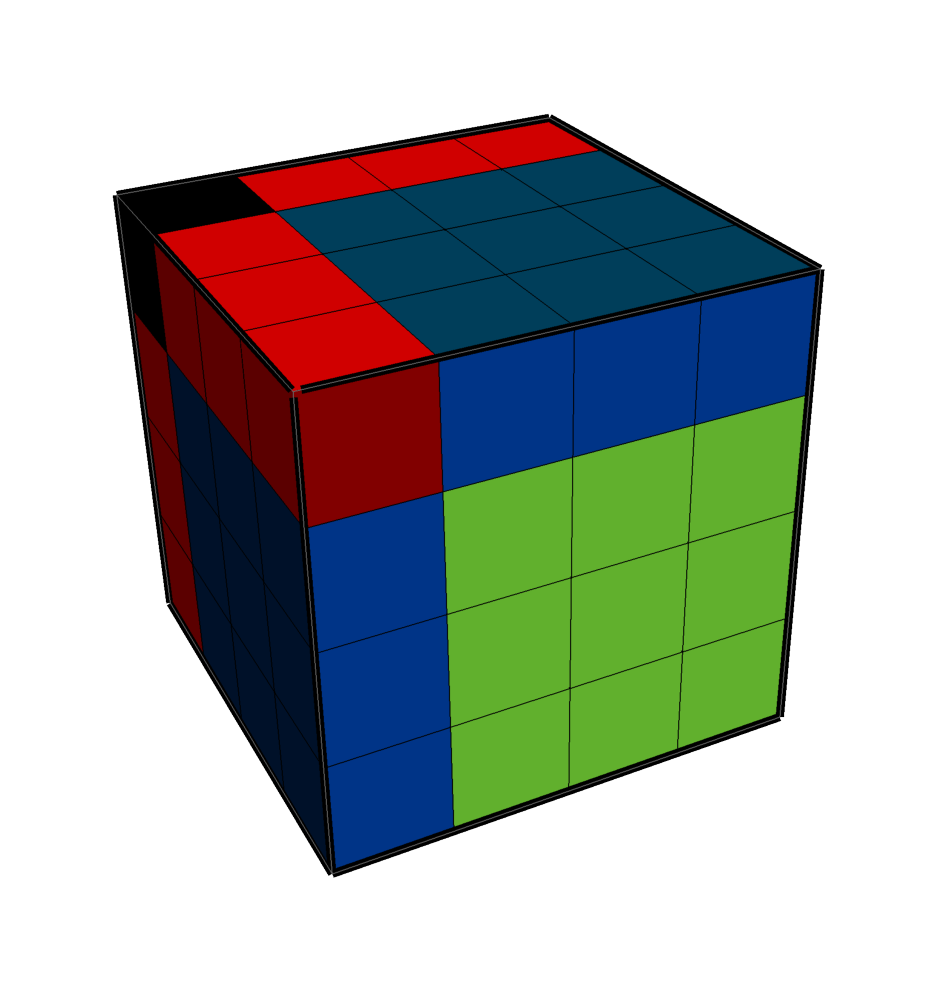
\includegraphics[height=3cm]{cubo_3qubits}
		\caption{}
	\end{subfigure}
	\caption{De izquierda a derecha se muestra la representación de la operación
	identidad de 1, 2 y 3 qubits. Llamaremos a esta representación las figuras PCE
  las operaciones PCE. Cada posición de un cuadrito o cubo, en el caso de una
  figura PCE de 3 qubits, está asociada con los subíndices $j_1,\ldots,j_n$ de 
  los elementos $\taus$ de la operación PCE. Si la posición $j_1,\ldots,j_n$ en 
  la figura PCE está pintado de color, entonces el elemento asociado $\taus$ es 
  igual a 1, y si la posición no está pintada, entonces el elemento asociado $\taus$ 
  es igual a 0. \ep}
	\label{fig:PCE_figs}
\end{figure} % }}}

%\esqueleto{Para una operación PCE de 2 qubits, los dos índices en las $\tau$
%sugieren que ahora la figura asociada debería ser de dos dimensiones. Así, 
%los tableritos representan a estas operaciones. Figuritas para explicar y demás.}

En la \Fref{fig:PCE_figs_examples} mostramos algunos ejemplos de figuras PCE. 
En la \Fref{fig:PCE_figs_examples_a} mostramos todas las figuras PCE de todas 
las operaciones PCE de 1 qubit; de izquierda a derecha, la operación identidad, las 
3 operaciones que mapean la esfera de Bloch a un disco perpendicular a cada
eje rectangular, las 3 operaciones que mapean la esfera de Bloch a una linea
sobre cada eje rectangular y la operación que mapea la esfera 
de Bloch al origen de coordenadas. En la \Fref{fig:PCE_figs_examples_b}
se muestran dos figuras PCE de operaciones que dejan invariantes
los conjuntos de componentes de Pauli $\{r_{00},r_{12},r_{21},r_{33}\}$ y 
$\{r_{00},r_{02},r_{10},r_{2,2},r_{32}\}$. Y en la 
\Fref{fig:PCE_figs_examples_c} se muestran dos operaciones PCE de 3 qubits
que dejan invariantes los conjuntos de componentes de Pauli $\{r_{000},
r_{300}, r_{033}\}$ y $\{r_{000},r_{220},r_{122}, r_{331}\}$.
Nótese que todas las figuras PCE que acabamos de discutir  
tienen pintado el cuadro o cubo con la posición $(0)$, $(0,0)$ o $(0,0,0)$.
Esto es así para todas las figuras PCE porque, de acuerdo con la definición 
\eqref{eq:PCE_definition}, una operación PCE preserva la traza de 
la matriz de densidad (\textit{i.e.} $\tau_{0,\ldots,0}=1$).
\begin{figure} % {{{
	\centering
	\begin{subfigure}[b]{0.48\textwidth}
		\centering
		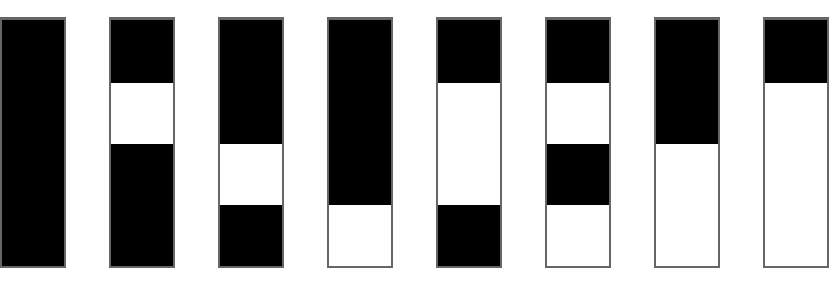
\includegraphics[height=2.5cm]	{1qubit_PCEOperations}
		\caption{}
		\label{fig:PCE_figs_examples_a}
	\end{subfigure}
	\hfill
	\begin{subfigure}[b]{0.48\textwidth}
		\centering
		\hfill 
		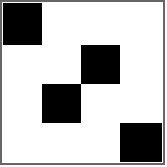
\includegraphics[height=2.3cm]{2qubits_pceChannel_example01} 
		\hfill
		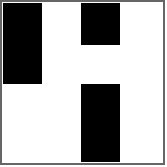
\includegraphics[height=2.3cm]{2qubits_pce_example}		
		\hfill \hfill
		\caption{}
		\label{fig:PCE_figs_examples_b}
	\end{subfigure}
	\newline
	\begin{subfigure}[c]{\textwidth}
		\centering
		\hspace*{\fill}
		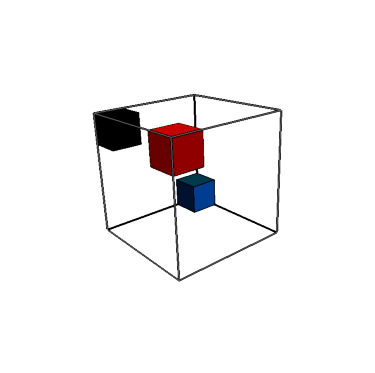
\includegraphics[width=4cm]{3qubits_PCE_ex1}
		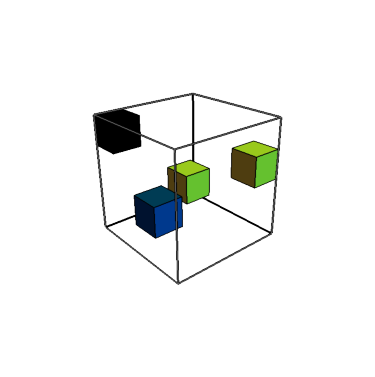
\includegraphics[width=4cm]{3qubits_PCE_ex2}
		\hspace*{\fill}
		\caption{}
		\label{fig:PCE_figs_examples_c}
	\end{subfigure}
	\caption{(a) Figuras PCE de todas las operaciones PCE de 1 qubit. 
	(b) Figuras PCE de 2 operaciones PCE de 2 qubits aleatorias. La primera 
	figura PCE representa a un canal PCE y la segunda representa una operación 
	PCE que no satisface la condición de completa positividad. \ep}
	\label{fig:PCE_figs_examples}
\end{figure} % }}}

\noindent
\esqueleto{En este punto, ya es más o menos obvio cómo es la representación 
geométrica de 3 qubits y que a partir de 4 qubits ya no podremos utilizar 
esta herramienta geométrica. Mostrar algunas figuras de PCEs de 3 qubits
y hablar de cómo hacer diferencia entre correlaciones y componentes 
locales en esas figuras según los colores 
(sólo para 3 qubits, porque las de 1 y 2 qubits 
las voy a poner en negro).}

\noindent
\esqueleto{Armados con esta potente herramienta geométrica, ahora 
es mucho más sencillo ganar intuición de las operaciones PCE e inferir 
características de los canales PCE. Entonces ahora mostraré los resultados 
de la sección anterior, pero usando las figuritas.}

Ahora mostramos de nuevo los resultados de los canales PCE de 2 qubits 
que presentamos en la \Tref{tab:2qubitsPCEChannel1sAnd0s},pero utilizando 
nuestra nueva representación de las figuras PCE, en la
\Fref{fig:2qubits_PCEChannels_figs}.
\begin{figure}
\centering
\begin{subfigure}[b]{0.49\textwidth}
	\centering
		
\includegraphics[height=1.4cm]{C1}
		\caption{C$\subind{1}{}$}
	\end{subfigure} \\
	\begin{subfigure}[b]{0.49\textwidth}
	\centering
		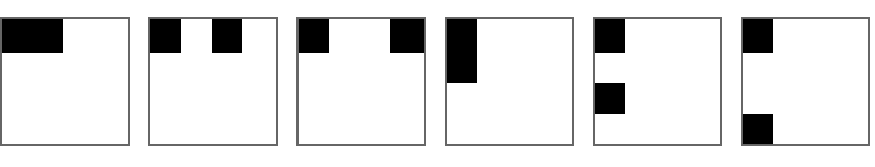
\includegraphics[height=1.4cm]{C2_1}
		\caption{C$\subind{2}{1}$}
	\end{subfigure}
	\begin{subfigure}[b]{0.49\textwidth}
		\centering
		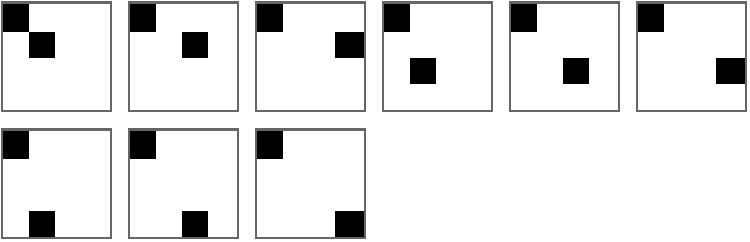
\includegraphics[height=2.4cm]{C2_2}
		\caption{C$\subind{2}{2}$}
	\end{subfigure}
	\begin{subfigure}[B]{0.49\textwidth}
		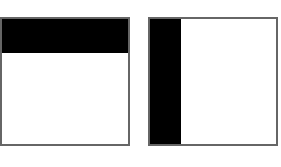
\includegraphics[height=1.4cm]{C4_1}
		\caption{C$\subind{4}{1}$}
	\end{subfigure}
	\begin{subfigure}[B][3.1cm]{0.49\textwidth}
	\centering
		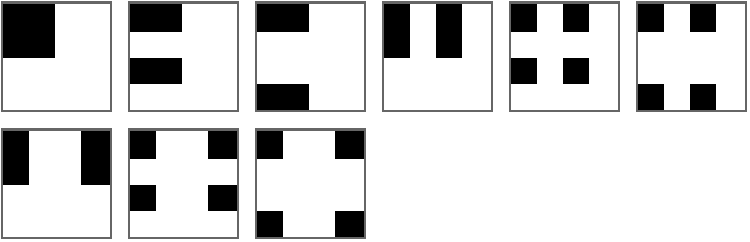
\includegraphics[height=2.4cm]{C4_2}
		\caption{C$\subind{4}{2}$}
	\end{subfigure}
	\begin{subfigure}[B]{0.49\textwidth}
		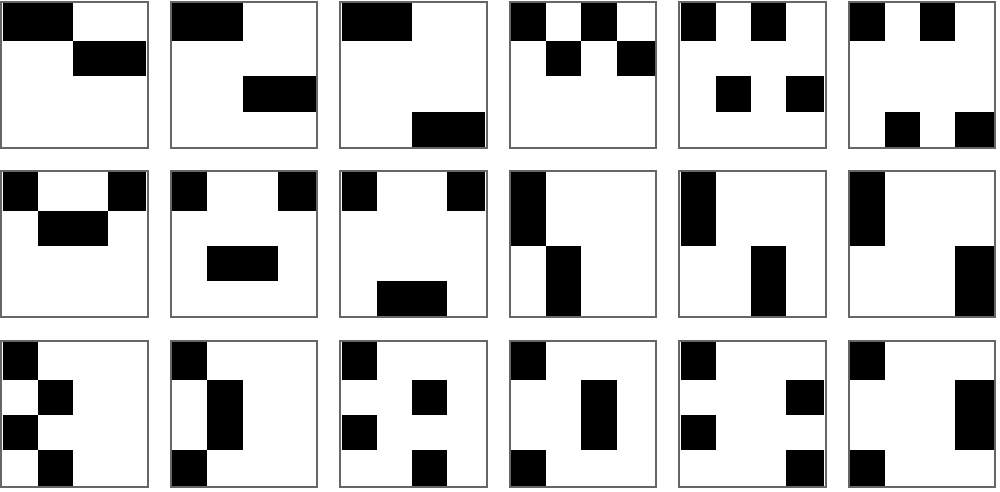
\includegraphics[height=3.6cm]{C4_3}
		\caption{C$\subind{4}{3}$}
	\end{subfigure}
	\begin{subfigure}[B][5.1cm]{0.49\textwidth}
		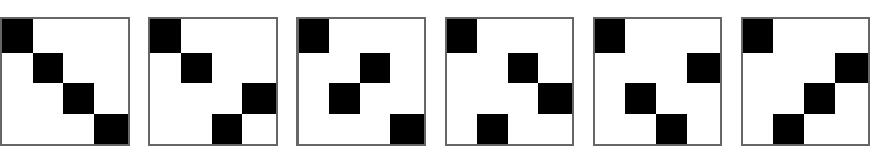
\includegraphics[height=1.4cm]{C4_4}
		\caption{C$\subind{4}{4}$}
	\end{subfigure}
	\begin{subfigure}[T]{0.49\textwidth}
		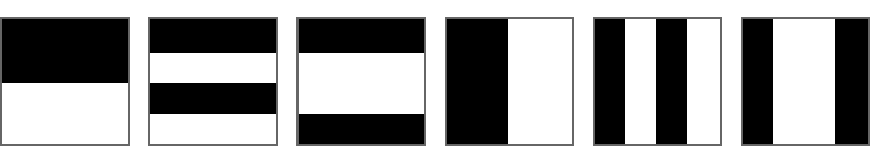
\includegraphics[height=1.4cm]{C8_1}
		\caption{C$\subind{8}{1}$}
	\end{subfigure}
	\begin{subfigure}[T][5.1cm]{0.49\textwidth}
		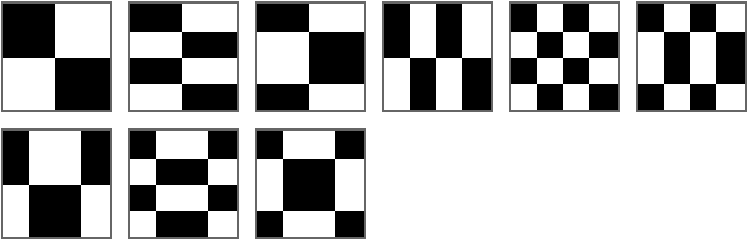
\includegraphics[height=2.4cm]{C8_2}
		\caption{C$\subind{8}{2}$}
	\end{subfigure}
	\begin{subfigure}[T]{0.49\textwidth}
	\centering
		
\includegraphics[height=1.4cm]{C16}
		\caption{C$\subind{16}{}$}
	\end{subfigure}
	\caption{Figuras PCE de los canales cuánticos PCE de 2 qubits ordenados por 
	clases de equivalencia etiquetadas como C$\subind{k}{l}$, donde $k$ es el número 
	de componentes de Pauli invariantes y $l$ es para diferenciar entre clases 
	de equivalencia con el mismo número de componentes de Pauli invariantes.}
	\label{fig:2qubits_PCEChannels_figs}
\end{figure} \vfill

\begin{figure}
	\centering
	\begin{subfigure}[T]{\textwidth}
		\centering
		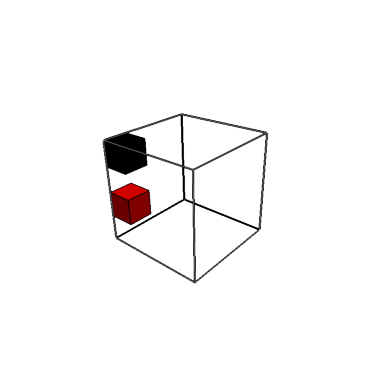
\includegraphics[width=4cm]{3q_2c_1} \hfill
		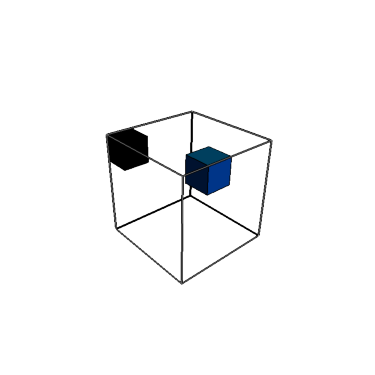
\includegraphics[width=4cm]{3q_2c_2} \hfill
		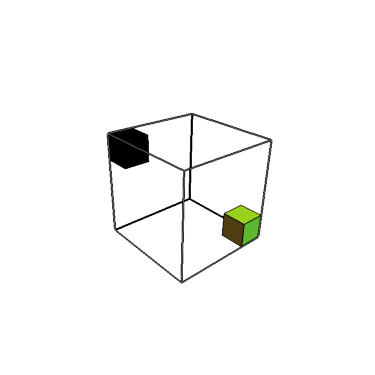
\includegraphics[width=4cm]{3q_2c_3}
		\caption{Elementos representativos de las 3 clases de equivalencia.}
	\end{subfigure}
	\begin{subfigure}[T]{\textwidth}
		\centering
		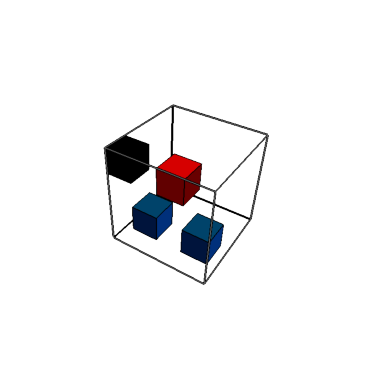
\includegraphics[width=4cm]{3q_1} \hfill
		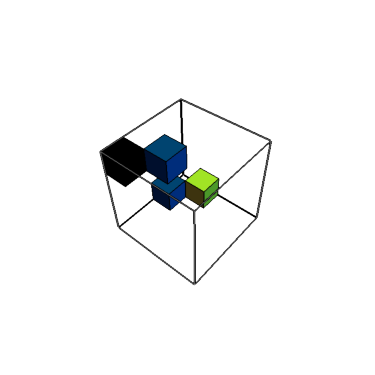
\includegraphics[width=4cm]{3q_2} \hfill
		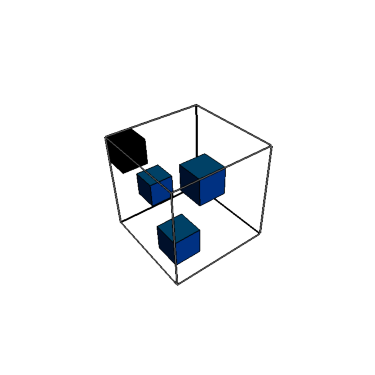
\includegraphics[width=4cm]{3q_3} \hfill
		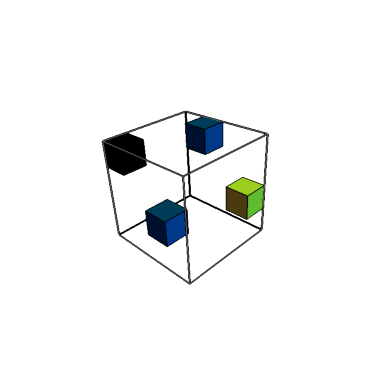
\includegraphics[width=4cm]{3q_4} \hfill
		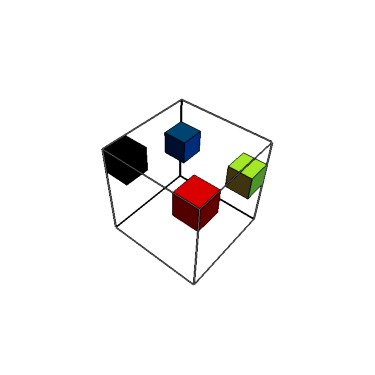
\includegraphics[width=4cm]{3q_5} \hfill
		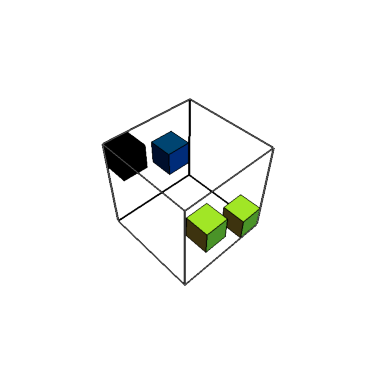
\includegraphics[width=4cm]{3q_6} 
		\caption{Canales PCE de 3 qubits que dejan invariantes 4 componentes de Pauli.}
	\end{subfigure}
	\caption{Figuras PCE de los canales cuánticos PCE de 3 qubits.}
\end{figure}

\section{Discusión de resultados}\label{sec:ch3_discussion}
\janote{Con el fin de hacer más eficiente la redacción, voy a partir del 
documento que preparamos para Sergey (justo coincide los resultados
que iban ahí con lo que vamos a poner en la tesis) y voy a iterar.}

\esqueleto{Esta sección es la que posee el contenido más importante 
de este manuscrito, después de la motivación y planteamiento del 
problema. Después de esta sección, lo único que haremos será 
estudiar si las operaciones PCE son un subconjunto de otras operaciones 
que fueron estudiadas por Ruskai.}

\esqueleto{Las figuras de los canales PCE exhiben patrones que todos 
comparten, parecen respetar alguna simetría...}

\esqueleto{Todos los canales PCE obedecen la regla de $2^k$...}

\esqueleto{Existen familias de canales PCE equivalentes. En las figuritas, 
esto se ve como transposiciones y permutaciones de filas y columnas. 
Físicamente, estos son swaps de partículas y cambios de base local.
Aquí yo creería que vale la pena discutir en palabritas, como en el documento
para sergey, pero también echarle algunas expresiones matemáticas como 
la de aplicar un swap, el PCE, y otro swap, por ejemplo...}

\esqueleto{La familia más sencilla de analizar es la de los PCE de 1 qubit
que dejan dos componentes de Pauli invariantes. Todos se pueden entender 
como la misma operación, pero conectados por rotaciones.}

\esqueleto{Hay correspondencia en el número de canales PCE que 
dejan $2^k$ y $2^{2n-k}$ componentes de Pauli invariantes.}

\esqueleto{Amarrado a la correspondencia de ``arcoiris'' van las reglas 
empíricas que formulamos con Alejo. Esta es otra prueba empírica que 
respalda la hipótesis de una conexión/correspondencia entre canales PCE.}

\esqueleto{Listo, hagamos un resumen de las características puntuales 
que inferimos de los canales PCE: ta ta ta.... Ahora sólo nos hace falta 
formalizar todo esto y hacer conexión formal entre todas las características. 
Además, sería deseable buscar alternativas para poder 
explorar numéricamente el caso completo de 3 e incluso de 4 qubits.}